\documentclass{amsart}

%%%%%%%%%%%%%%%%%%%%%%%%%%%%%%%%%%%%%%

\usepackage[utf8]{inputenc}
\usepackage[T1]{fontenc}

\usepackage{a4wide}%en grand
\usepackage{changepage}%indentation

\usepackage{xcolor}
\usepackage{amsfonts, amsthm, amssymb, amsmath}
\usepackage{mathtools}
\usepackage{wasysym}
\usepackage{xspace}
\usepackage{graphicx}
\usepackage[notcite,notref]{showkeys} % shows labels 
%\usepackage{breqn}
\usepackage{algorithm}
\usepackage{algorithmic}
\usepackage{tabularx}

\usepackage[english]{babel} %gestion des langues
\usepackage{caption}
\usepackage{subcaption}
\usepackage{paralist, enumerate}
\usepackage{multirow}

\usepackage{hyperref}
\hypersetup{colorlinks=true, citecolor=darkblue, linkcolor=darkblue}
\usepackage{hypcap}

\usepackage[noabbrev,capitalise]{cleveref}
%\usepackage{autonum}
\usepackage{xspace}

%%%%%%%%%%%%%%%%%%%%%%%%%%%%%%%%%%%%%%

\newtheorem{theorem}{Theorem}[section]
\newtheorem{proposition}[theorem]{Proposition}
\newtheorem{lemma}[theorem]{Lemma}
\newtheorem{ce}[theorem]{Counter-example}
\newtheorem{claim}[theorem]{Claim}
\newtheorem{corollary}[theorem]{Corollary}
\newtheorem{definition}[theorem]{Definition}
\newtheorem{conjecture}[theorem]{Conjecture}
\newtheorem{notation}[theorem]{Notation}
\theoremstyle{remark}
\newtheorem{remark}[theorem]{Remark}
\newtheorem{example}[theorem]{Example}
\newtheorem{algo}{Algorithm}
\newtheorem*{example*}{Example}

\crefname{theorem}{Theorem}{Theorems}
\crefname{lemma}{Lemma}{Lemmas}
\crefname{conjecture}{Conjecture}{Conjectures}

\definecolor{darkblue}{rgb}{0,0,0.7} % darkblue color
\newcommand{\darkblue}{\color{darkblue}} % darkblue command
\newcommand{\defn}[1]{\textsl{\darkblue #1}} % emphasis of a definition

%%%%%%%%%%%%%%%%%%%%%%%%%%%%%%%%%%%%%%

% math special letters
\newcommand{\R}{\mathbb{R}} % reals
\newcommand{\N}{\mathbb{N}} % naturals
\newcommand{\Z}{\mathbb{Z}} % integers
\newcommand{\C}{\mathbb{C}} % complex
\newcommand{\disk}{\mathbb{D}} % disk

% math commands
\newcommand{\set}[2]{\left\{ #1 \;\middle|\; #2 \right\}} % set notation
\newcommand{\bigset}[2]{\big\{ #1 \;\big|\; #2 \big\}} % big set notation
\newcommand{\Bigset}[2]{\Big\{ #1 \;\Big|\; #2 \Big\}} % Big set notation
\newcommand{\setangle}[2]{\left\langle #1 \;\middle|\; #2 \right\rangle} % set notation
\newcommand{\ssm}{\smallsetminus} % small set minus
\newcommand{\dotprod}[2]{\left\langle \, #1 \; \middle| \; #2 \, \right\rangle} % dot product
\newcommand{\symdif}{\,\triangle\,} % symmetric difference
\newcommand{\one}{{1\!\!1}} % the all one vector
\newcommand{\eqdef}{\mbox{\,\raisebox{0.2ex}{\scriptsize\ensuremath{\mathrm:}}\ensuremath{=}\,}} % :=
\newcommand{\defeq}{\mbox{~\ensuremath{=}\raisebox{0.2ex}{\scriptsize\ensuremath{\mathrm:}} }} % =:
\newcommand{\viceversa}{\textit{vice versa}} % vice versa

\newcommand*{\dual}[1]{{#1^*}}
\newcommand*{\nbd}[0]{neighbourhood\xspace}
\newcommand*{\ef}[0]{E-finite\xspace}
\newcommand*{\vf}[0]{V-finite\xspace}
\newcommand*{\ktg}[0]{$k$-triangulation\xspace}

\newcommand{\cl}{\prec}
\newcommand{\cle}{\preccurlyeq}

\newcommand{\surface}{\mathcal{S}}
\newcommand{\cylinder}{\mathcal{C}}

\graphicspath{{../figures/}}

\newcommand{\ie}{\textit{i.e.}~} % id est
\newcommand{\eg}{\textit{e.g.}~} % exempli gratia

% marginal comments
\usepackage{todonotes}
\newcommand{\vincent}[1]{\todo[color=blue!30]{#1 \\ \hfill --- V.}}
\newcommand{\mathias}[1]{\todo[color=red!30]{#1 \\ \hfill --- M.}}

%%%%%%%%%%%%%%%%%%%%%%%%%%%%%%%%%%%%%%

\title[Infinite multitriangulations of a disk and multitriangulations of surfaces]{Infinite multitriangulations of a disk \\ and multitriangulations of surfaces}

\thanks{ML was partially supported by the French ANR grant GATO~(16\,CE40\,0009). \\ \indent VP was partially supported by the French ANR grants SC3A~(15\,CE40\,0004\,01) and CAPPS~(17\,CE40\,0018).}

\author{Mathias Lepoutre}
\address{LIX, \'Ecole Polytechnique, Palaiseau}
\email{mathias.lepoutre@lix.polytechnique.fr}
\urladdr{\url{http://www.lix.polytechnique.fr/Labo/Mathias.Lepoutre/}}

\author{Vincent Pilaud}
\address{CNRS \& LIX, \'Ecole Polytechnique, Palaiseau}
\email{vincent.pilaud@lix.polytechnique.fr}
\urladdr{\url{http://www.lix.polytechnique.fr/~pilaud/}}

%%%%%%%%%%%%%%%%%%%%%%%%%%%%%%%%%%%%%%

\begin{document}

\begin{abstract}
This note partially extends the structural properties of $k$-stars and diagonal flips of $k$-triangulations on a convex polygon to the case of $k$-triangulations on any surface with marked points on the boundary. 
To that extent, we use the universal cover of the surface to transform a graph embedded on a surface into a periodic graph of an infinite polygon.
We generalize the work of V.~Pilaud and F.~Santos to $k$-triangulations of an infinite polygon with some weak additional constraints, and we finally derive properties of $k$-triangulations on any surface.
\end{abstract}

\vspace*{-.3cm}

\maketitle

%\begin{figure}[h]
%	\capstart
%	\centerline{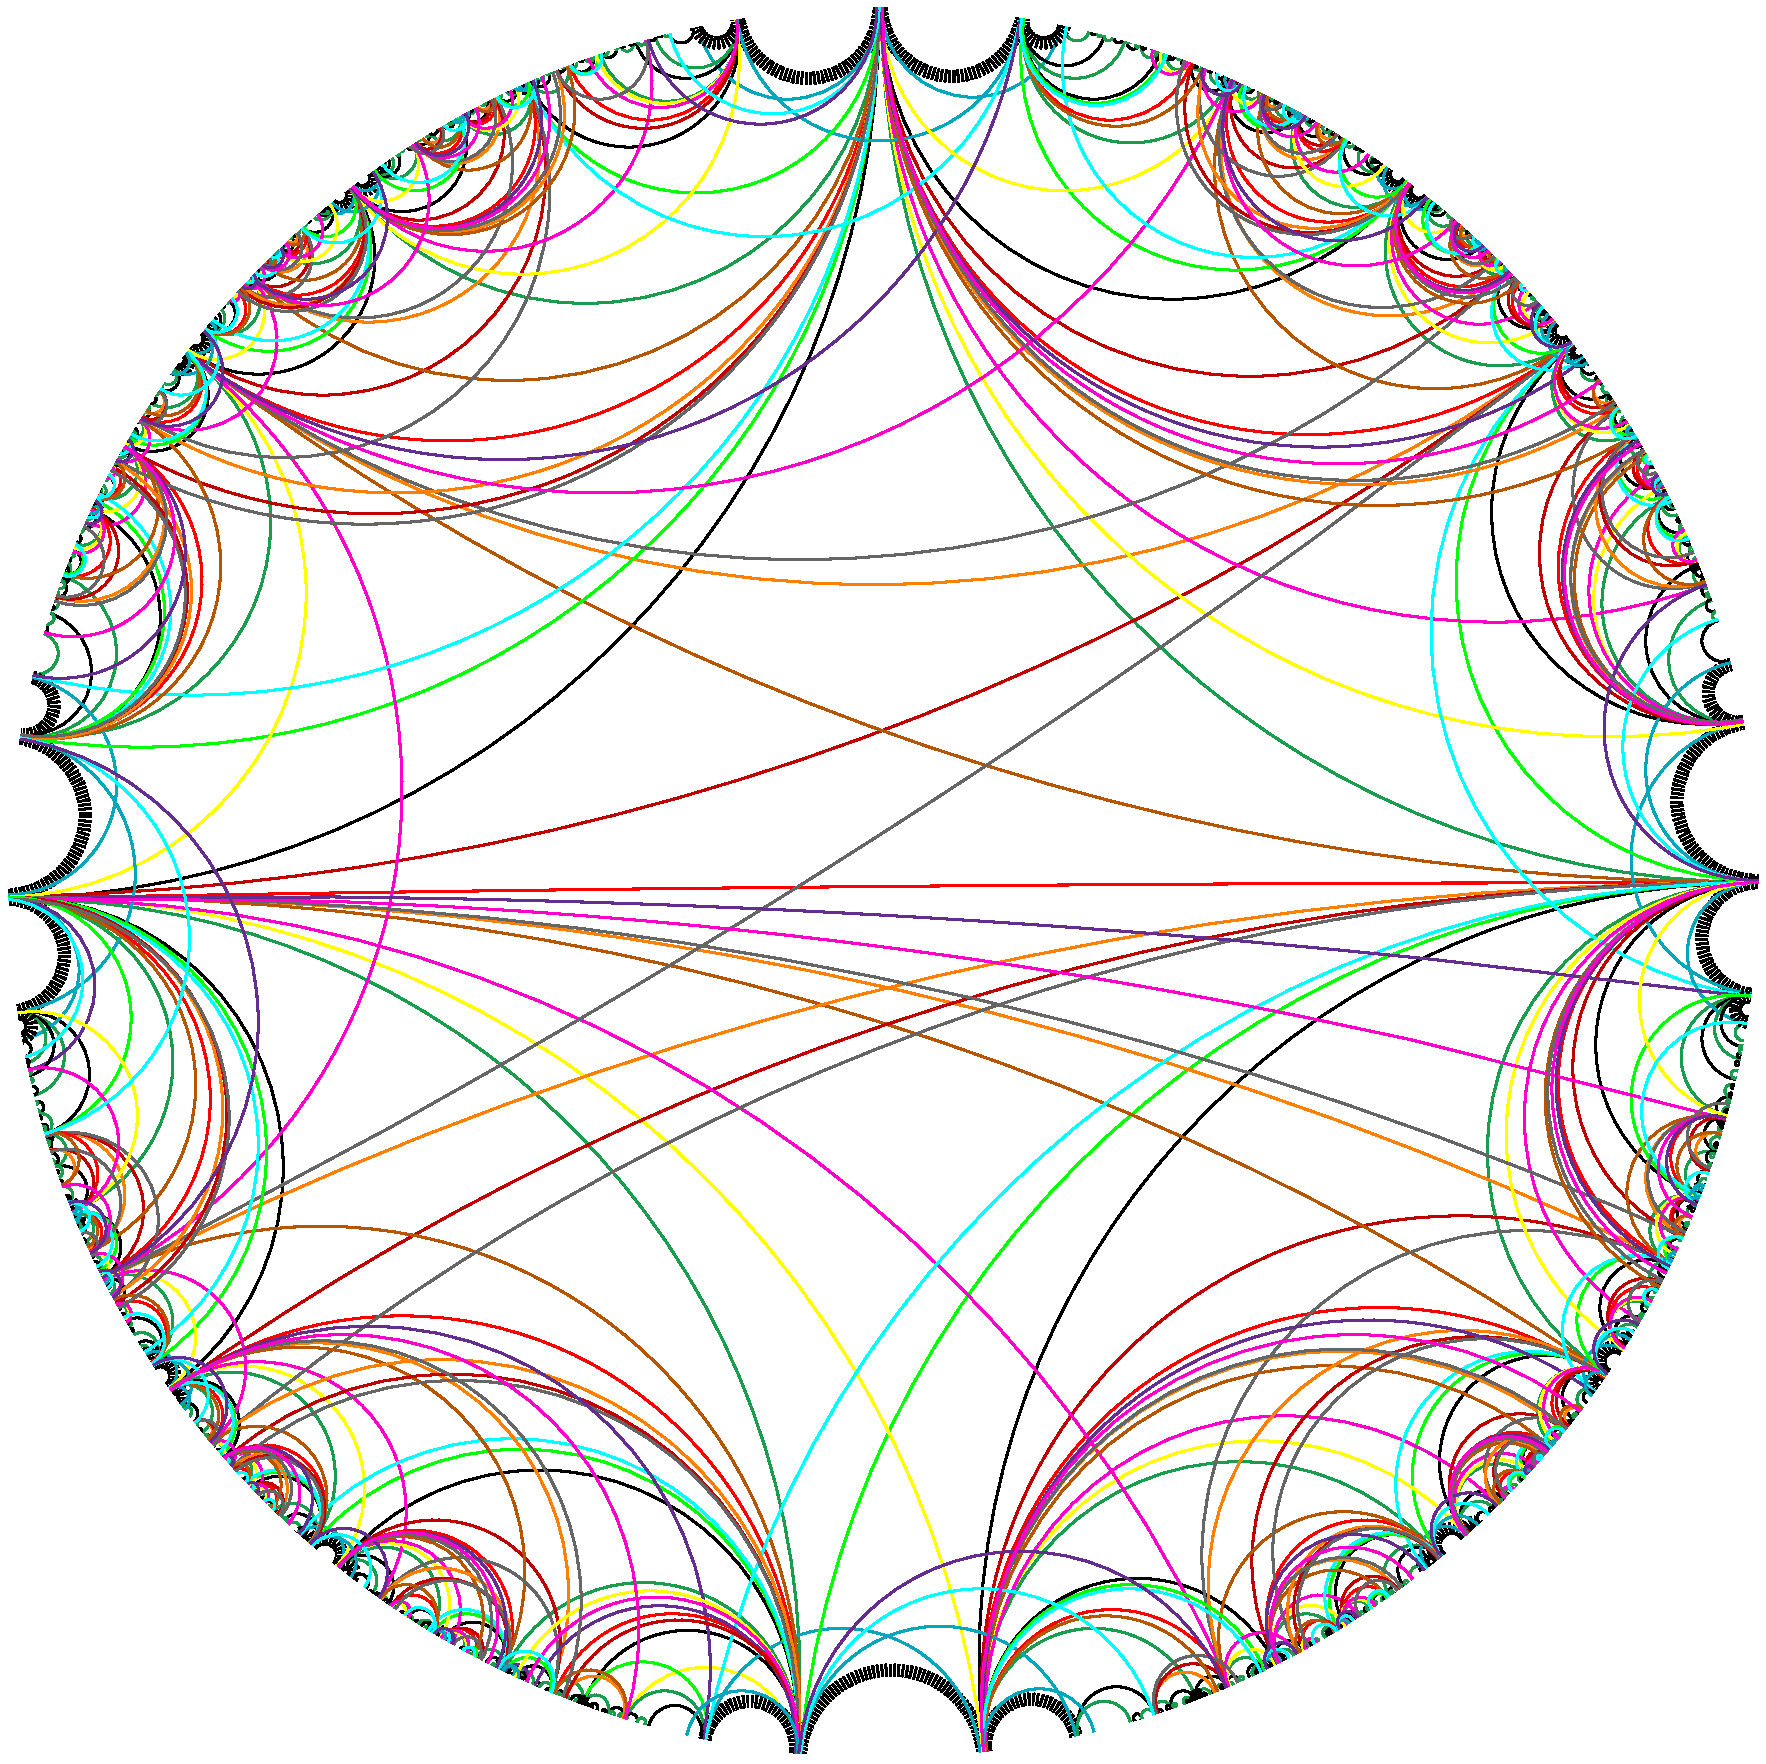
\includegraphics[scale=.42]{torus/torusEdges}}
%	\caption{The universal cover of the $2$-triangulation of a torus with one hole and one marked point, represented in \cref{fig:torus}. It has five $2$-stars and all flips are sequential.}
%	\label{fig:UCtorus}
%\end{figure}

Triangulations are fundamental tools to understand and manipulate topological spaces.
Triangulations of surfaces are particularly interesting as they feature strong enumerative and structural combinatorial properties.
On the enumerative side, triangulated maps on surfaces are counted by surprising product formulas. % line of research started analytically by W.~Tutte in the sixties and actively developed by bijective approaches.
On the structural side, crossing-free collections of arcs between marked points on a given surface form a pure and thin simplicial complex, whose facets are triangulations.
In particular, triangulations admit a natural flip operation that exchanges an arc~$a$ with the other diagonal of the quadrangle formed by the two triangles containing~$a$.
These structural properties were used for instance to provide a large and relevant family of examples of cluster algebras whose combinatorics is driven by the triangulations of a surface and the flips between~them.

Triangulations can be interpreted as maximal crossing-free collections of arcs connecting a fixed collection of marked points on the boundary of the surface.
An interesting line of research arises when considering maximal collections of arcs with ``few crossings''.
There are various relevant ways to restrict crossings.
One can require for instance that the arcs have at most $\ell$ crossings in total, or that there is no subset of $\ell+2$ mutually crossing arcs, or that each arc crosses at most $\ell$ other arcs, etc.
All these conditions translate natural restrictions forcing the intersection graph of the arcs to be a ``small graph''.
Namely, it corresponds to an intersection graph with at most $\ell$ edges, with no $(\ell+2)$-clique, or with maximal degree~$\ell$, etc.
Note that all these restrictions specialize to classical triangulations when~$\ell = 0$.
The first restriction (at most $\ell$ crossings) has been studied in details in~\cite{PilaudRue}.
In this note, we consider the second restriction (no subset of mutually crossing arcs), which were already considered in the literature in the case of a disk.

A \defn{$k$-triangulation} of a convex $n$-gon is a maximal set of diagonals with no $(k+1)$-crossing, \ie no subset of $k+1$ mutually crossing diagonals.
They were introduced in~\cite{CapoyleasPach} and particularly studied in~\cite{Nakamigawa, DressKoolenMoulton, Jonsson1, Jonsson2, SerranoStump, PilaudSantos-multitriangulations}.
They feature some strong structural properties, which naturally generalize classical properties of the triangulations of a convex polygon~($k=1$):
\begin{enumerate}[(i)]
\item All $k$-triangulations of the $n$-gon have $k(2n-2k-1)$ diagonals~\cite{CapoyleasPach, Nakamigawa, DressKoolenMoulton}.\mathias{j'ai changé cette formule de n à 2n}
\item Any diagonal of length at least~$k + 1$ can be flipped and the graph of flips is regular and connected~\cite{Nakamigawa, DressKoolenMoulton}.
\item Any $k$-triangulation decomposes into a complex of $k$-stars~\cite{PilaudSantos-multitriangulations}.
\item The set of $k$-triangulations of the $n$-gon is enumerated by a determinant of Catalan numbers~\cite{Jonsson1, Jonsson2}. It is thus in bijection with families of $k$ mutually non-crossing Dyck paths~\cite{SerranoStump}.
\end{enumerate}

The objective of this note is to introduce the good notion of $k$-triangulations on a surface such that properties (i) to (iii) above hold (note that, as there will be infinitely many $k$-triangulations as soon as the surface has at least~$1$ one handle or at least $2$ boundaries, the enumerative point~(iv) will naturally be lost).
For this, we start from a surface~$\surface$ with boundaries and fix some marked points on its boundaries.
We then consider collections of arcs (up to homotopy) joining marked points with no $(k+1)$-crossing.
The right notion of $(k+1)$-crossings requires to consider the universal cover~$\bar\surface$ of the surface~$\surface$.
Namely, a $(k+1)$-crossing in~$\surface$ is the projection of a set of $k+1$ mutually crossing arcs in the universal cover~$\bar\surface$.
The subtlety here is that there are collections of pairwise crossing arcs of~$\surface$ which do not admit pairwise crossing representatives on the universal cover~$\bar\surface$.
Armed with this solid notion of $k$-triangulations on~$\surface$, we are able to prove analogues of properties (i) and (iii) above, and to discuss property (ii).

In fact, our approach is to first consider $k$-triangulations on a disk with infinitely many vertices (see \cref{sec:infiniteMultitriangulations}).
Under rather weak assumptions that ensure a sort of local finiteness, we show that these infinite $k$-triangulations decompose into $k$-stars and admit a flip operation.
We then consider $k$-triangulations on surfaces as quotients of periodic infinite $k$-triangulations by Fuchsian groups (see \cref{sec:multitriangulationsSurfaces}).
Most structural properties of infinite triangulations are preserved by this quotient.
As discussed at the end of this note, the main difficulty remains in the behavior of the periodicity under the flip operation.

%%%%%%%%%%%%%%%%%%%%%%%%%%%%%%%%%%%%%%

\section{Multitriangulations of infinite polygons}
\label{sec:infiniteMultitriangulations}

The objective of this section is to study $k$-triangulations of an infinite polygon.
The key property here is the existence of the $k$-star decomposition established for $k$-triangulations of a convex $n$-gon in~\cite{PilaudSantos-multitriangulations}.
In fact, many arguments of~\cite{PilaudSantos-multitriangulations} easily adapt to the case of an infinite polygon assuming some sort of local finiteness properties that we present first.

%%%%%%%%%%%%

\subsection{Infinite polygons}

We now provide a proper definition of infinite polygon (\cref{def:infinitePolygon}) and of two local finiteness conditions (\cref{def:tidyPolygon,def:EV-finite}) that will be relevant later.

\begin{definition}
\label{def:infinitePolygon}
A \defn{polygon}~$P$ is a cyclically ordered set, that might be finite or infinite.
We write~$u \cl v \cl w$ for the cyclic order.
The elements of~$P$ are called \defn{points} and pairs of elements of~$P$ are called \defn{diagonals}.
For two points~$u,w \in P$, let~$[u,w] \eqdef \set{v \in P}{u \le v \le w}$, and define similarly the intervals~$[u,w[$, $]u,w]$ and~$]u,w[$ (with open brackets for strict inequalitites).
Two diagonals~$(t,u)$ and~$(v,w)$ of~$P$ \defn{cross} if~$t \cl v \cl u \cl w$ or $v \cl t \cl w \cl u$.
\end{definition}

\begin{definition}
\label{def:tidyPolygon}
If $u$ and $v$ are two points of a polygon~$P$ such that the interval~$]u,v[$ is empty, we say that~$u$ is the \defn{predecessor} of~$v$ and that~$v$ is the \defn{successor} of~$u$, and we use the notations~$v = u+1$ and~$u = v-1$. A polygon~$P$ is \defn{tidy} if each point of~$P$ has both a predecessor and a successor. In particular, finite polygons are tidy.
\end{definition}

In particular, note that a tidy polygon is \defn{discrete}, meaning that each of its points is isolated. However, the converse is not true. For instance, the subset $\{-1\}\cup \{1, \frac{1}{2},\frac{1}{3}\cdots\}$ of~$\R$ is discrete, but not tidy, since $-1$ has no successor.

\begin{definition}
\label{def:EV-finite}
A set~$D$ of diagonals of a polygon~$P$ is 
\begin{itemize}
\item \defn{\ef} if each diagonal of~$D$ is crossed by a finite number of diagonals of~$D$,
\item \defn{\vf} if each vertex of~$P$ is incident to finitely many diagonals of~$D$.
\end{itemize}
\end{definition}

%%%%%%%%%%%%

\subsection{Infinite multitriangulations}

We now define $k$-triangulations of infinite polygons exactly as those of finite convex polygons.

\begin{definition}
A \defn{$k$-crossing} of a polygon~$P$ is a set of~$k$ pairwise crossing diagonals of~$P$.
A \defn{$k$-triangulation} of~$P$ is an inclusion-maximal set of diagonals of~$P$ with no $(k+1)$-crossing.
\end{definition}

\begin{definition}
The \defn{length} of a diagonal~$(u,v)$ of a polygon~$P$ is the minimum~$\ell(u,v)$ of~$|{]u,v[}|$ and~$|{]u,v[}|$ (note that this might be infinite).
A diagonal~$(u,v)$ with~$\ell(u,v) > k$ (resp.~$\ell(u,v) = k$, resp.~$\ell(u,v) < k$) is a \defn{$k$-relevant} (resp.~\defn{$k$-boundary}, resp.~\defn{$k$-irrelevant}) diagonal.
\end{definition}

\begin{remark}
\label{rem:kboundary}
Observe that a diagonal contained in a $(k+1)$-crossing must be $k$-relevant.
Therefore, any \ktg contains all $k$-irrelevant and $k$-boundary diagonals by maximality.
\end{remark}

\begin{example}
\cref{fig:torusEdges} represents an example of a $2$-triangulation of an infinite tidy polygon.
In all pictures, we only represent diagonals until a certain depth, and we leave it to the reader to complete the picture when needed.

\begin{figure}[h]
	\capstart
	\centerline{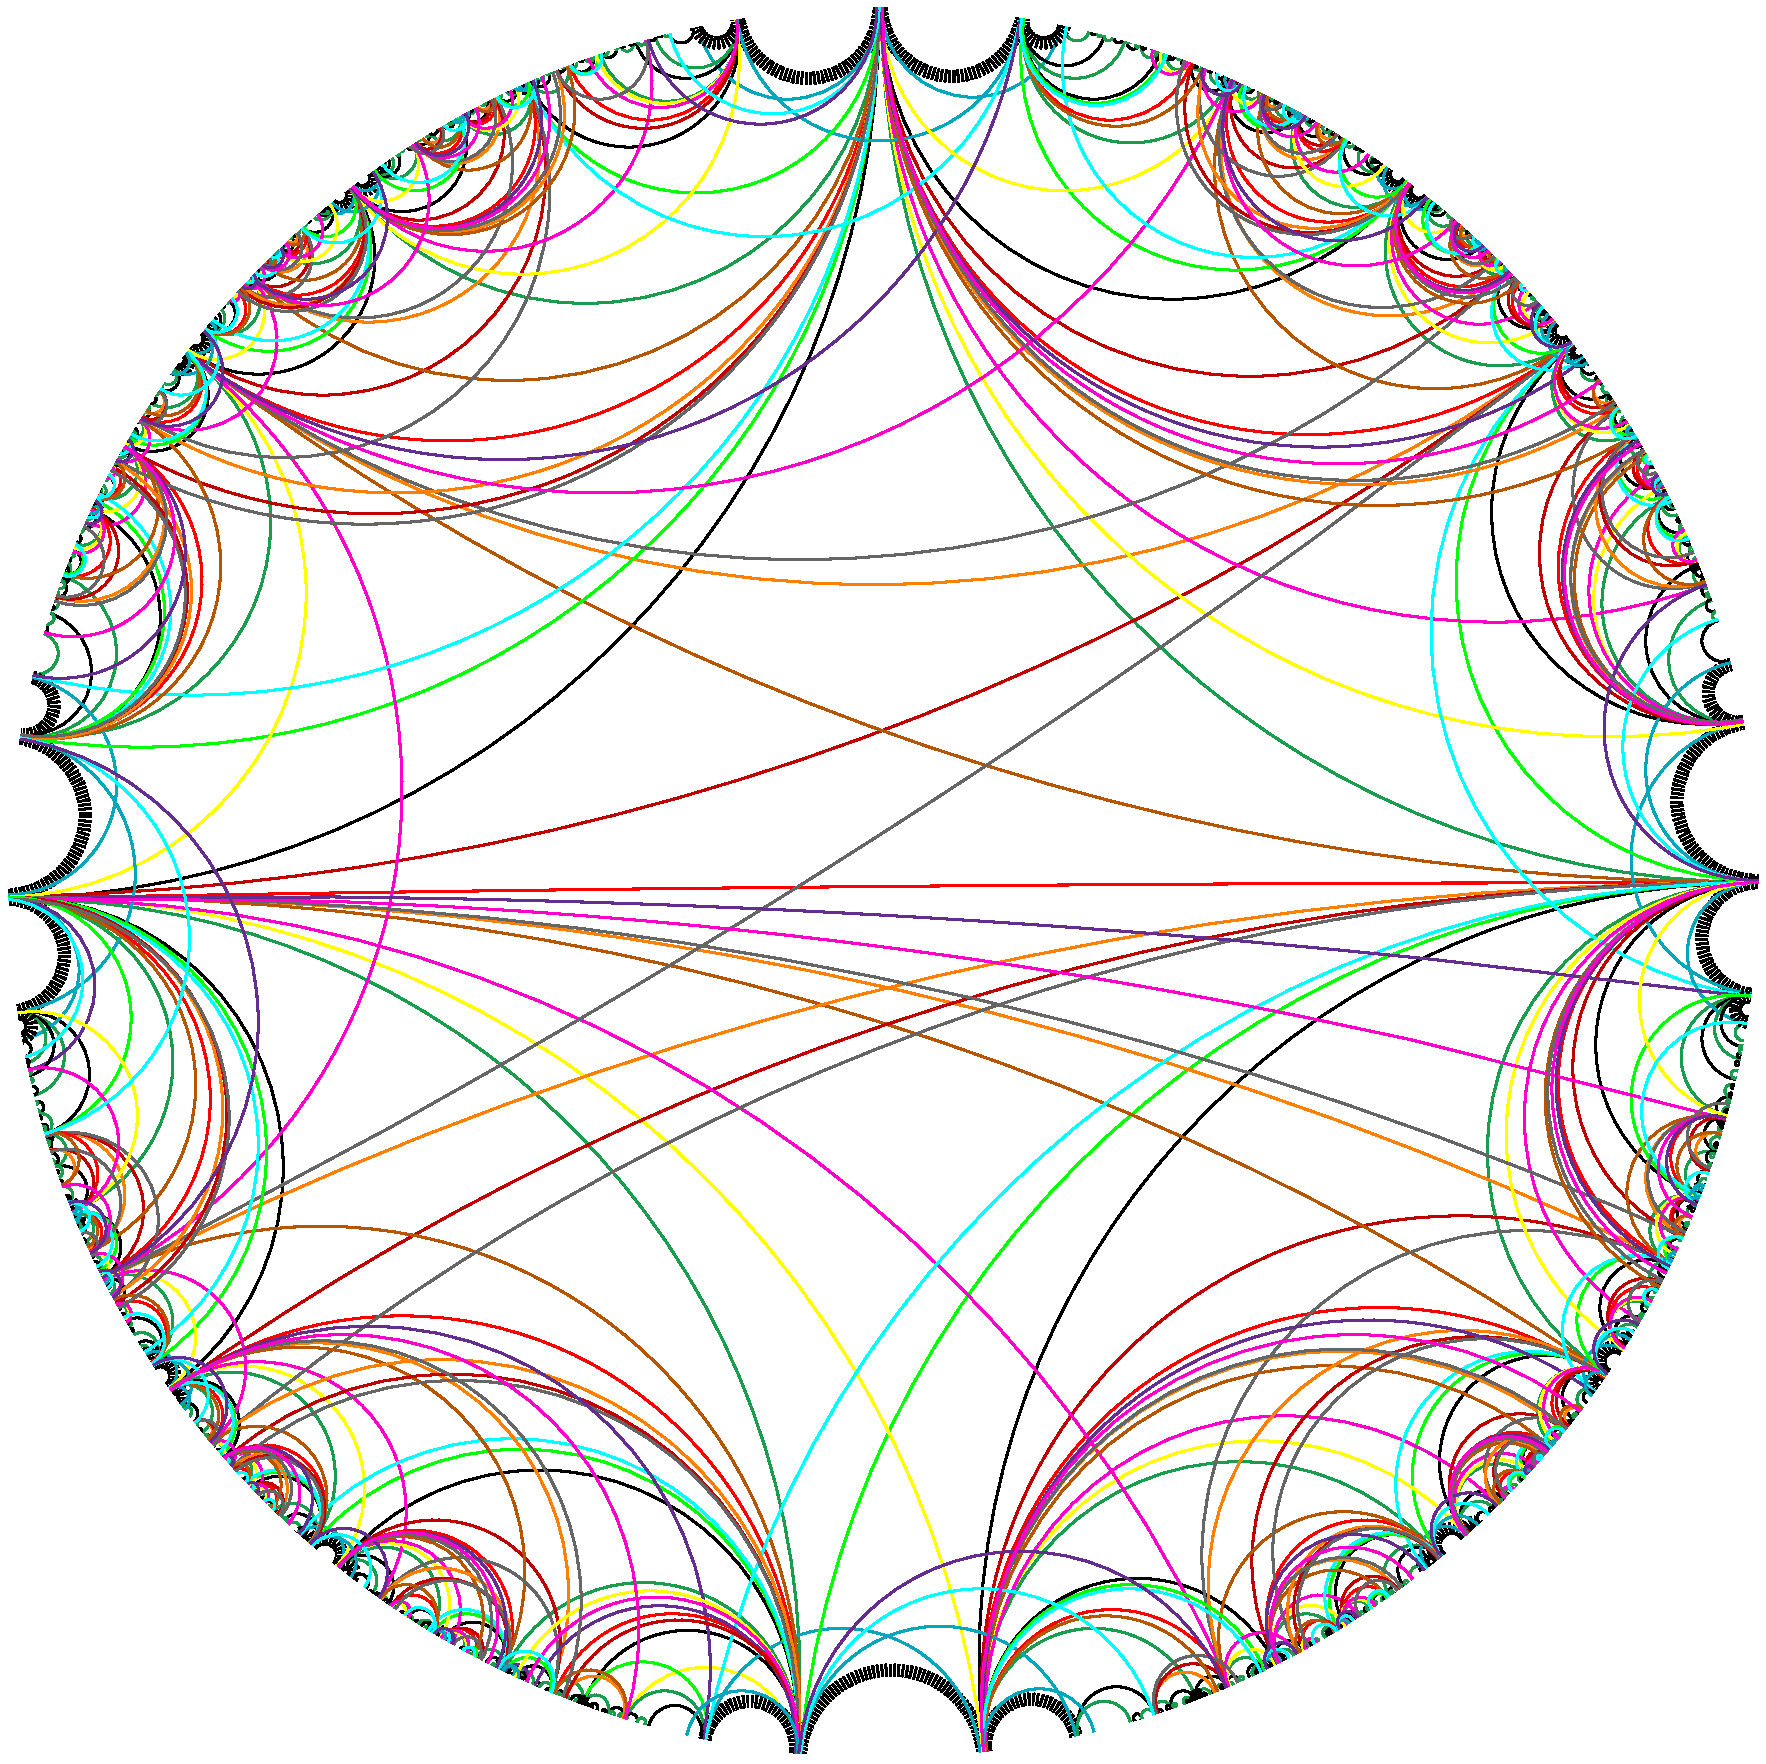
\includegraphics[scale=.42]{torus/torusEdges}}
	\caption{A $2$-triangulation of an infinite polygon.}
	\label{fig:torusEdges}
\end{figure}
\end{example}

As observed in~\cite{PilaudSantos-multitriangulations}, many combinatorial properties of $k$-triangulations are better understood from their decompositions into $k$-stars, which generalize triangles in triangulations.

\begin{definition}
A \defn{$k$-star} of a polygon~$P$ is a set~$S$ of diagonals of~$P$ of the form~$\set{(s_i, s_{i+k})}{0 \le i \le 2k}$ where~$s_0 \cl \dots \cl s_{2k}$ (where the indices are understood modulo~$2k+1$).
\end{definition}

\begin{definition}
An \defn{angle} of a set~$D$ of diagonals of a polygon~$P$ is a pair of diagonals~$\{(u,v), (v,w)\}$ with~$u \cl v \cl w$ such that~$D$ contains no diagonal of the form~$(v,t)$ with~$w \cl t \cl u$. The angle is denoted by~$\angle(u,v,w)$ and we say that~$v$ is the \defn{apex} of~$\angle(u,v,w)$. An angle is \defn{$k$-relevant} if its two diagonals are $k$-relevant or $k$-boundary diagonals. %A set~$Y$ of diagonals of~$P$ crosses the angle~$\angle(u,v,w)$ if each diagonal of~$Y$ crosses both~$(u,v)$ and~$(v,w)$. 
\end{definition}

One of the objectives of this paper is to prove the following structural results on infinite $k$-triangulations.

\begin{theorem}
\label{thm:structureInfinite}
Let~$T$ be a \ef \ktg of a tidy polygon~$P$. Then:
\begin{enumerate}
\item Each $k$-relevant angle of~$T$ is contained in precisely one $k$-star of~$T$.
\item Each $k$-relevant (resp.~$k$-boundary, resp.~$k$-irrelevant) diagonal of~$T$ is contained in precisely two (resp.~one, resp.~no) $k$-stars of~$T$.
\item For any $k$-relevant diagonal~$e$ of~$T$, there exists a unique diagonal~$f$ not in~$T$ such that~$T \symdif \{e,f\}$ is another $k$-triangulation (where~$\symdif$ denotes the symmetric difference). Moreover, the diagonal~$f$ only depend on the two $k$-stars of~$T$ containing~$e$.
\item Let~$P'$ denote a polygon obtained by replacing $k+1$ consecutive points of~$P$ by~$k$ points. Then there exists a flattening (resp.~inflating) operation that transforms the \ktg{}s of~$P$ into the \ktg{}s of~$P'$ (resp.~and \viceversa).
%\item For any point~$p$ of the plane, the $k$-depth of~$p$ in~$P$ is equal to the sum of the winding numbers around~$p$ of the $k$-stars of~$T$.
\end{enumerate}
\end{theorem}

\begin{example}
\cref{fig:torusStars} shows the decomposition into $2$-stars of the $2$-triangulation of \cref{fig:torusEdges}.

\begin{figure}[h]
	\capstart
	\centerline{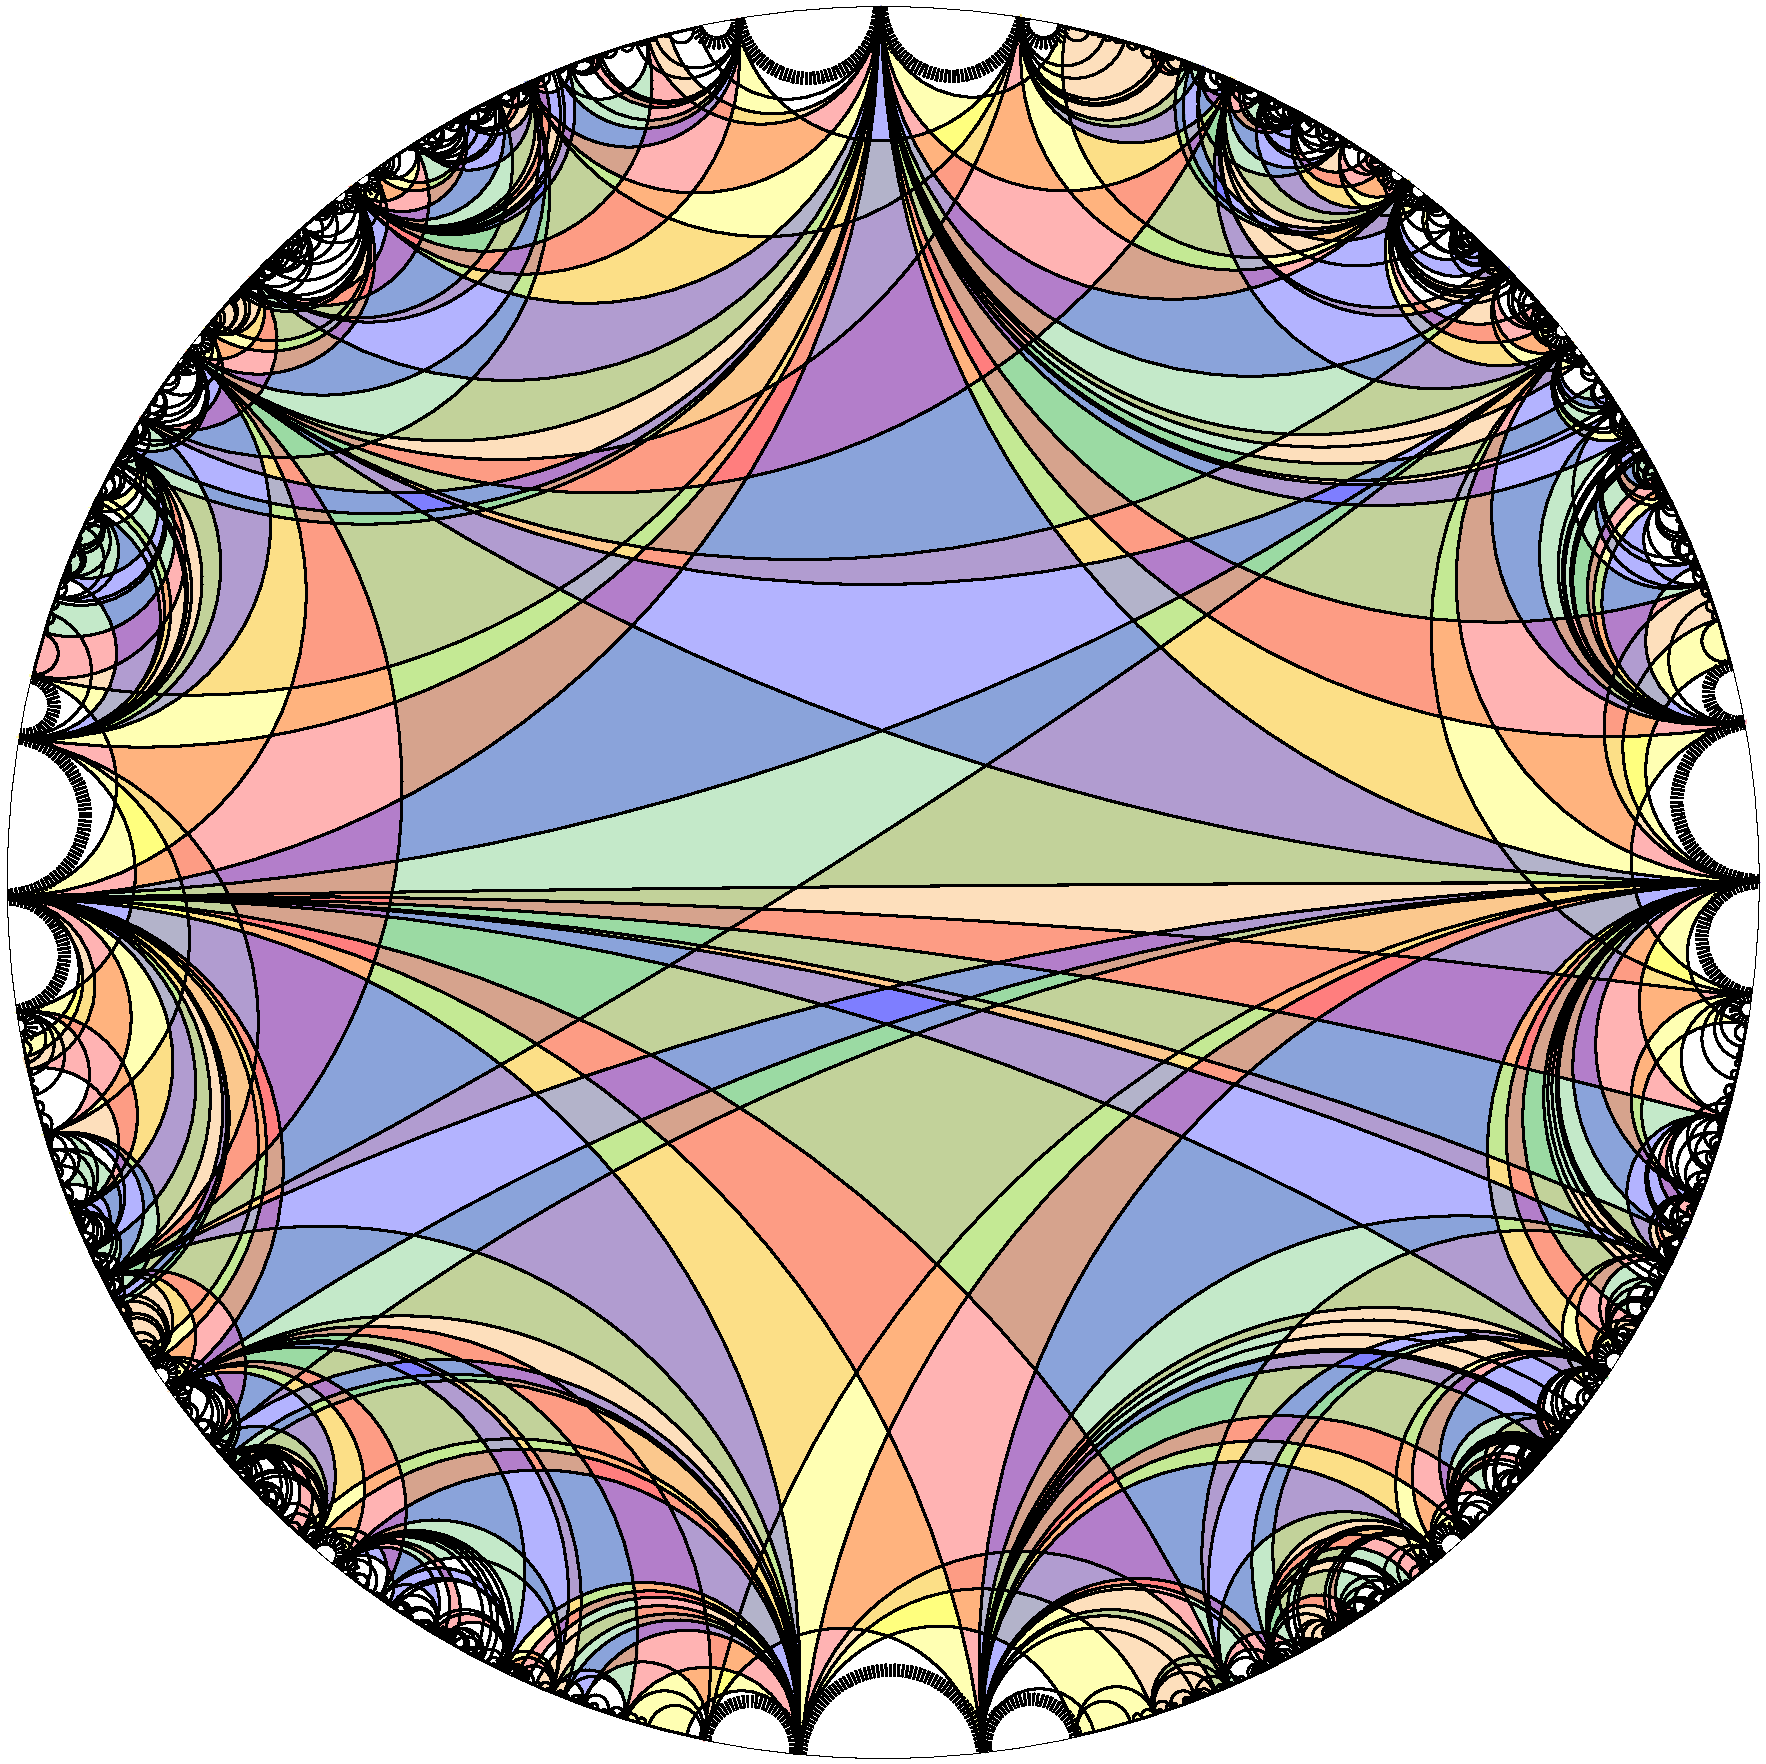
\includegraphics[scale=.42]{torus/torusStars}}
	\caption{The decomposition into $2$-stars of the $2$-triangulation of \cref{fig:torusEdges}.}
	\label{fig:torusStars}
\end{figure}
\end{example}

%We prove \cref{thm:structureInfinite} in \cref{subsec:prfInfinite}.
%
%\begin{remark}
%\begin{itemize}
%\item flip graph connected? Increasing flip graph?
%\item duality with pseudoline arrangements?
%\item $k$-arboresence? connection to $k$-edge-connected but not locally $(k+1)$-edge-connected.
%\end{itemize}
%\end{remark}

%%%%%%%%%%%%

%\subsection{Some counter-examples}
%
%\begin{ce}
%The polygon of a periodic \ktg is not necessarily a \nbd.
%\end{ce}
%\begin{proof}
%
%\end{proof}
%
%\begin{ce}
%A periodic \ef \ktg may have angles that are not crossed by a $(k-1)$-crossing.
%\end{ce}
%\begin{proof}
%
%\end{proof}
%
%\begin{ce} 
%A periodic \ktg may not be \ef.
%\end{ce}
%\begin{proof}
%
%\end{proof}
%
%\begin{ce}
%A \ef \ktg of a \nbd is not necessarily \vf.
%\end{ce}
%\begin{proof}
%k=1
%\end{proof}

%%%%%%%%%%%%

\subsection{Proof of \cref{thm:structureInfinite}}
\label{subsec:prfInfinite}

The end of this section is devoted to the proof of \cref{thm:structureInfinite}.
We follow the ideas of the proof of~\cite{PilaudSantos-multitriangulations} in the case of finite convex polygons, but we adapt the arguments to show that the conditions of $E$-finiteness and tidiness suffice to obtain the same result in the case of infinite polygons.

%%%

\subsubsection{$(k-1)$-crossings crossing an angle}

We first study the $(k-1)$-crossings that cross a given angle in a $k$-triangulation.

\begin{definition}
A $(k-1)$-crossing~$A = \{a_1, \dots, a_{k-1}\}$ \defn{crosses} an angle~$\angle(u,v,w)$ if each diagonal~$a_i$ crosses both diagonals~$(u,v)$ and~$(v,w)$.
\end{definition}

We stick to the convention to label the diagonals of~$A$ by~$a_i \eqdef (a^\bullet_i, a^\circ_i)$ in such a way that $u \cl a^\bullet_1 \cl \dots \cl a^\bullet_{k-1} \cl v \cl a^\circ_1 \cl \dots \cl a^\circ_{k-1} \cl w$. We use this convention throughout this section without further notice.

\begin{lemma}
\label{lem:tidyExists}
In a \ktg $T$ of a tidy polygon, any $k$-relevant angle is crossed by a $(k-1)$-crossing.
\end{lemma}

\begin{proof}
Any angle~$\angle(u,v,w)$ is crossed by the $(k-1)$-crossing~$\set{(v-k+i, v+i)}{i \in [k-1]}$ of $k$-boundary diagonals, which belongs to the \ktg $T$ by \cref{rem:kboundary}.
\end{proof}

\begin{definition}
Let $\angle(u,v,w)$ be a $k$-relevant angle of $T$.
For two diagonals~$a$ and~$b$ of $T$ that cross $\angle(u,v,w)$, we say that $a$ is \defn{$v$-farther} than $b$ if $u \cl a^\bullet \cle b^\bullet \cl v \cl b^\circ \cle a^\circ \cl w$. For two $(k-1)$-crossings $A = \{a_1, \dots, a_{k-1}\}$ and $B = \{b_1, \dots, b_{k-1}\}$ that cross $\angle(u,v,w)$, we say that $A$ is \defn{$v$-farther} than $B$ if $a_i$ is $v$-farther than $b_i$ for every $i \in [k-1]$. We say that $A$ is the \defn{$v$-farthest} $(k-1)$-crossing if it is $v$-farther than any other $(k-1)$-crossing that crosses~$\angle(u,v,w)$.
\end{definition}

\begin{lemma}
In a \ktg, the set of $(k-1)$-crossings crossing a given $k$-relevant angle forms a distributive lattice.
\end{lemma}

\begin{proof}
Consider two $(k-1)$-crossings $A = \{a_1, \dots, a_{k-1}\}$ and $B = \{b_1, \dots, b_{k-1}\}$ that cross the angle~$(u,v,w)$.

There is no $i$ such that $a_i$ crosses $b_i$. 
Indeed, suppose $a^\bullet_i \cl b^\bullet_i \cl v \cl a^\circ_i \cl b^\circ_i$. Then $\{(u, v), a_1, \dots, a_i, b_i, \dots, b_{k-1}\}$ forms a $(k+1)$-crossing. 
Similarly, if $b^\bullet_i \cl a^\bullet_i \cl v \cl b^\circ_i \cl a^\circ_i$, then $\{(u, v), b_1, \dots, b_i, a_i, \dots, a_{k-1}\}$ forms a $(k+1)$-crossings.
Hence $A$ and $B$ are edgewise comparable.

We define the meet (resp.~join) of $A$ and $B$ as their edgewise minimum (resp.~maximum). With this definition it is easy to see that we obtain a distributive lattice.
\end{proof}

\begin{lemma}
\label{lem:efMax}
In a \ef \ktg, for any angle~$\angle(u,v,w)$ crossed by at least one $(k-1)$-crossing, there exists a $v$-farthest $(k-1)$-crossing that crosses~$\angle(u,v,w)$.
\end{lemma}

\begin{proof}
By \ef{}ness, the angle~$\angle(u,v,w)$ is crossed by a finite number of $(k-1)$-crossings. Hence the distributive lattice of such $(k-1)$-crossings is finite, and has a unique maximum.
\end{proof}

Combining \cref{lem:tidyExists,lem:efMax}, we obtain the following statement.

\begin{corollary}
\label{coro:farthestTidy}
In a \ef \ktg of a tidy polygon, for any angle~$\angle(u,v,w)$, there exists a $v$-farthest $(k-1)$-crossing that crosses~$\angle(u,v,w)$.
\end{corollary}

%%%

\subsubsection{Any $k$-relevant angle belongs to a $k$-star}

We now use the existence of a $v$-farthest $(k-1)$-crossing to show that the angle~$\angle(u,v,w)$ belongs to a $k$-star.

\begin{proposition}
\label{prop:angleBelongStar}
For any angle~$\angle(u,v,w)$ of a \ktg, if there is a $v$-farthest $(k-1)$-crossing that crosses~$\angle(u,v,w)$, then~$\angle(u,v,w)$ belongs to a $k$-star.
\end{proposition}

\begin{proof}
The proof follows the same lines as that of~\cite[Thm.~4.1]{PilaudSantos-multitriangulations}. We repeat the argument here for the convenience of the reader.

Let $E=\{e_1, \dots , e_{k-1}\}$ be the $v$-farthest $(k-1)$-crossing that crosses $\angle(u, v, w)$.
We will prove that the diagonals $(u, e^\circ_1), (e^\bullet_1, e^\circ_2) \dots (e^\bullet_{k-2}, e^\circ_{k-1}), (e^\bullet_{k-1}, w)$ are in $T$ such that the points $u$, $e^\bullet_1, \dots, e^\bullet_{k-1}$, $v$, $e^\circ_1, \dots, e^\circ_{k-1}$, $w$ are the vertices of a $k$-star of $T$ containing the angle $\angle(u, v, w)$. 

To get this result, we use two steps, illustrated in \cref{fig:exProofStar}: first we prove that $\angle(e^\bullet_1, e^\circ_1, u)$ is an angle of $T$, and then we prove that the diagonals $e_2, \dots, e_{k-1}, (v, w)$ form a $(k-1)$-crossing intersecting $\angle(e^\bullet_1, e^\circ_1, u)$ and $e^\circ_1$-farthest (so that we can reiterate the argument).


\begin{figure}
  \centering
  \begin{subfigure}[b]{.48\textwidth}
	\centering
	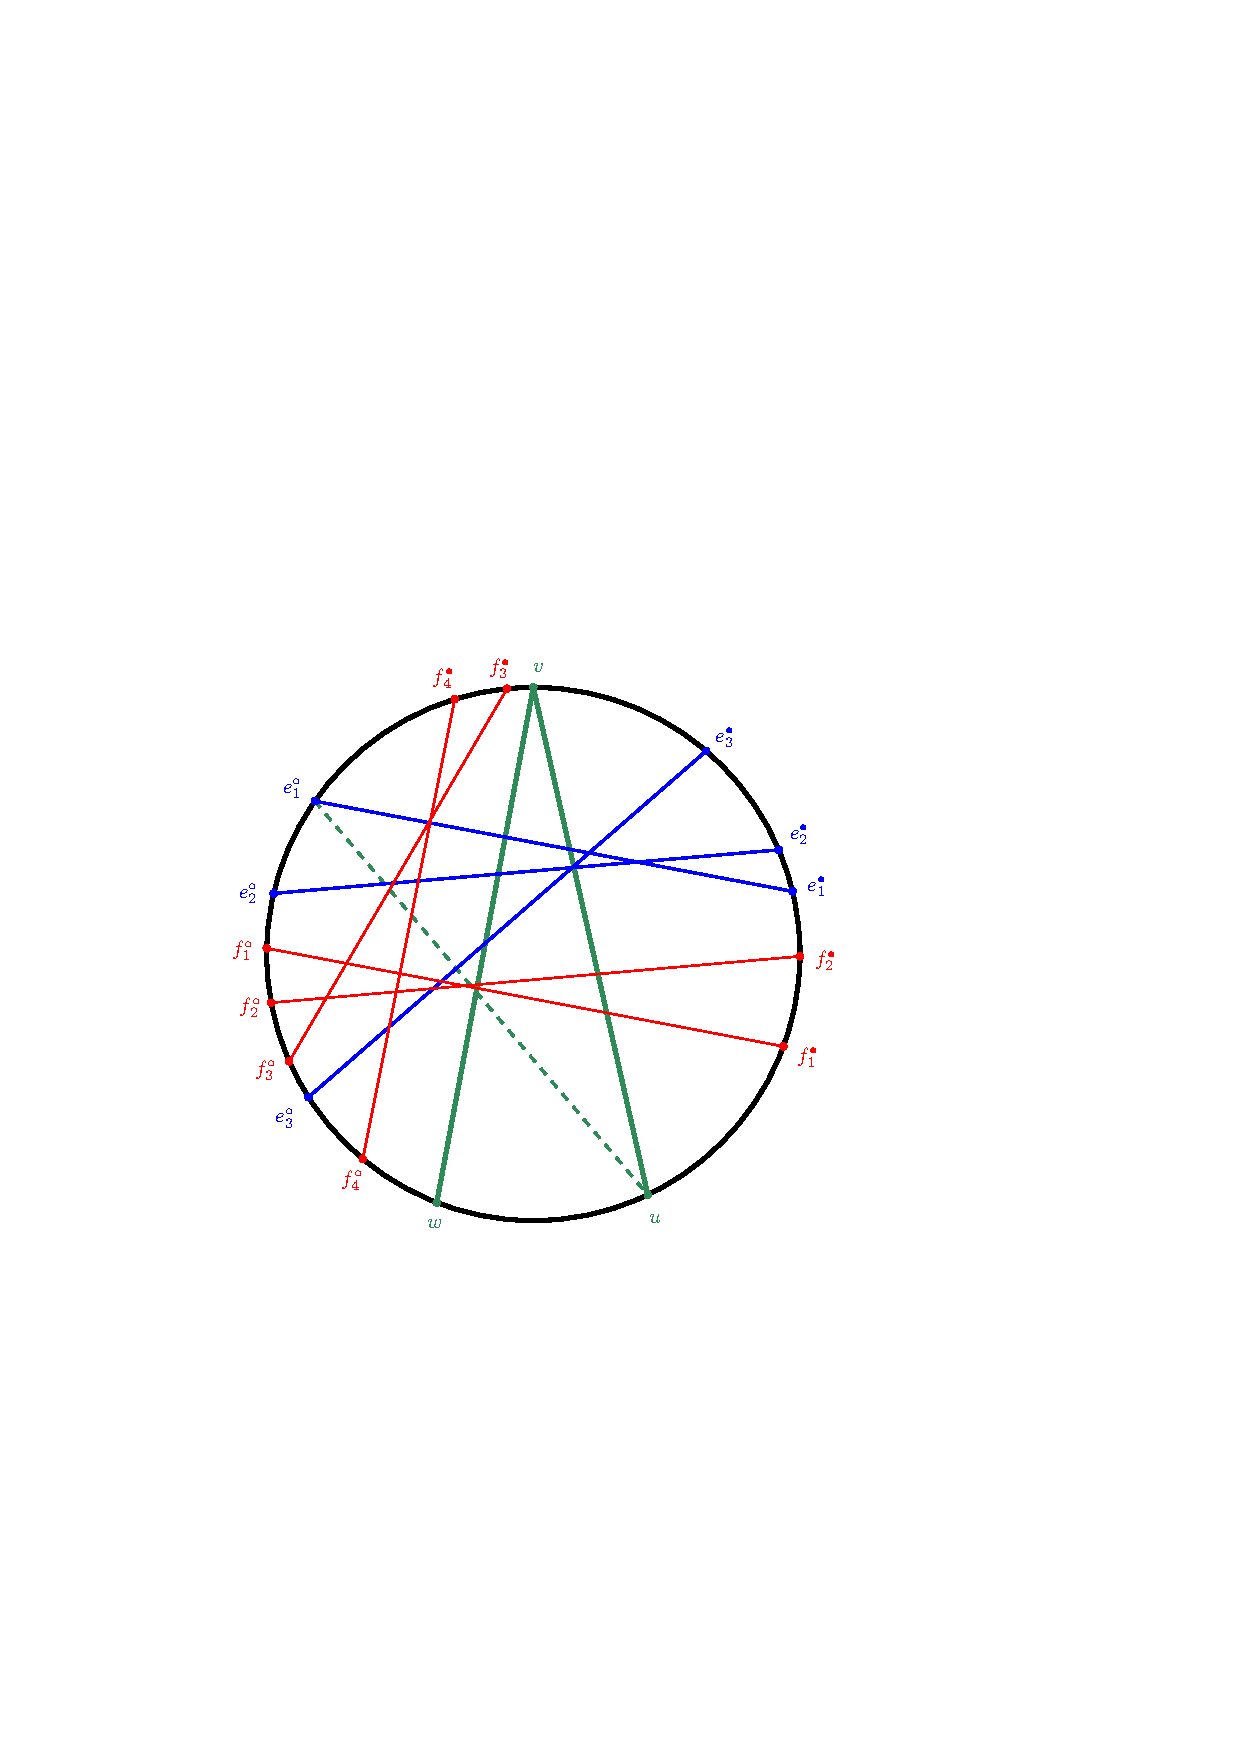
\includegraphics[width=\textwidth,page=1]{exProofStar}
  \end{subfigure}
  \begin{subfigure}[b]{.48\textwidth}
    \centering
    \includegraphics[width=\textwidth,page=2]{exProofStar}
  \end{subfigure}
  \caption{Illustrations of the first and second steps of the proof of \cref{prop:angleBelongStar}. In both case, $k=4$, and on the left, $\ell=2$.}
  \label{fig:exProofStar}
\end{figure}

\medskip
\paragraph{\bf First step.}
Suppose that $(u, e^\circ_1)$ is not in $T$. 
Since $T$ is a $k$-triangulation, there is a $k$-crossing $F=\{f_1, \dots, f_k\}$ (with $u \cl f^\bullet_1 \cl \cdots \cl f_k \cl e'_1 \cl f'_1 \cl \cdots \cl f'_k \cl u$) that prevents the diagonal~$(u, e^\circ_1)$. We will now exhibit a $(k-1)$-crossing of the form~$\{f_1, \dots, f_\ell, e_{\ell+1}, \dots, e_{k-1}\}$ that will cross~$\angle(u,v,w)$ and be $v$-farther than~$E$, contradicting the maximality of~$E$.

Note first that~$f^\bullet_k \in [v, e^\circ_1[$, as otherwise~$F \cup \{(u, v)\}$ would form a $(k + 1)$-crossing.
Additionnaly, $f^\circ_k \in {]e^\circ_1, w]}$, as otherwise $E \cup \{(v,w), (f^\bullet_k, f^\circ_k)\}$ would form a $(k + 1)$-crossing. 
Consequently, we have~$f^\circ_1 \in {]e^\circ_1, w[}$ $e^\circ_1 \cl f^\circ_1 \cl \cdots \cl f^\circ_{k-1} \cl w$.

Let $\ell = \max \set{j\in[k-1]}{\, f^\circ_i \in {]e^\circ_i, w[} \text{ for all } i \le j}$.
Then $f^\bullet_i \in {]u, e^\bullet_i]}$ for any $i \le \ell$, as otherwise $\{e_1, \dots , e_i, f_i, \dots , f_k\}$ would form a $(k + 1)$-crossing.
Thus~$f_i$ crosses~$\angle(u,v,w)$ and is $v$-farther than~$e_i$ for any~$i \le \ell$.
Furthermore, we have $f^\circ_\ell \cl f^\circ_{\ell+1} \cl e^\circ_{\ell+1}$ (by maximality of~$\ell$) and~$f^\bullet_\ell \cl e^\bullet_{\ell} \cl e^\bullet_{\ell+1}$, so that~$f_\ell$ crosses~
$e_{\ell+1}$. 
Consequently, we get a $(k-1)$-crossing $\{f_1, \dots , f_\ell, e_{\ell+1}, \dots , e_{k-1}\}$ which is $v$-farther than $\{e_1, \dots , e_{k-1}\}$, contradicting the maximality of~$E$. 
We conclude that~$(u, e^\circ_1)$ belongs to~$T$.

Suppose now that~$\angle(e^\bullet_1, e^\circ_1, u)$ is not an angle of~$T$. 
Then there exists $e^\bullet_0 \in {]u, e^\bullet_1[}$ such that $(e^\bullet_0, e^\circ_1) \in T$. 
But then the $(k-1)$-crossing $\{(e^\bullet_0, e^\circ_1), e_2, \dots, e_{k-1}\}$ is $v$-farther than~$E$. 
This implies that~$\angle(e^\bullet_1, e^\circ_1, u)$ is an angle of~$T$.

\medskip
\paragraph{\bf Second step.}
Assume now that there exists a $(k-1)$-crossing~$F=\{f_2, \dots , f_k\}$ that crosses $\angle(e^\bullet_1, e^\circ_1, u)$ and is $e^\circ_1$-farther than the $(k-1)$-crossing $\{e_2, \dots, e_{k-1}, (v, w)\}$.

Note first that~$f_k = (v,w)$. Indeed, since~$f_k$ is $e^\circ_1$-farther than~$(v,w)$, we have~$f^\bullet_k \in {]e^\bullet_1, v]}$ and~$f^\circ_k \in [w,u[$. Therefore~$f^\bullet_k = v$ (as otherwise~$\{(u,v), e_1\} \cup F$ would form a $(k+1)$-crossing), and~$f^\circ_k = w$ (since~$\angle(u,v,w)$ is an angle of~$T$).

Since~$f_k = (v,w)$, we obtain that~$\{e_1, f_2, \dots, f_{k-1}\}$ is a $(k-1)$-crossing that crosses~$\angle(u,v,w)$. For any $i \in [2,k-1]$, the diagonal~$f_i$ is $e^\circ_1$-farther than~$e_i$, and thus also $v$-farther than~$e_i$. Therefore, $\{e_1, f_2, \dots, f_{k-1}\}$ is $v$-farther than~$E$, contradicting the maximality of~$E$.
\end{proof}

Combining \cref{coro:farthestTidy} and \cref{prop:angleBelongStar}, we obtain the proof of \cref{thm:structureInfinite}\,(1).

\begin{corollary}
\label{coro:angleInStar}
In a \ef \ktg of a tidy polygon, any $k$-relevant angle belongs to a $k$-star.
\end{corollary}

%%%

\subsubsection{Any $k$-relevant diagonal belongs to two $k$-stars}

We now use $k$-relevant angles to show that any $k$-relevant (resp.~$k$-boundary, resp.~$k$-irrelevant) diagonal of a $k$-triangulation~$T$ is contained in precisely two (resp.~one, resp.~no) $k$-stars of~$T$.

\begin{lemma}
When $k \ge 2$, any \ef \ktg of a tidy polygon is also \vf.
\end{lemma}

\begin{proof}
Any $k$-boundary diagonal~$e$ surrounding a given vertex~$v$ intersects all diagonals adjacent to~$v$.
As the $k$-triangulation is \ef, the diagonal~$e$ intersects finitely many diagonals, thus~$v$ has finite degree.
Note that the reverse implication is wrong: there are \vf $k$-triangulations that are not \ef.
\end{proof}

\begin{lemma}
\label{lem:diagsInAngles}
Any $k$-relevant (resp.~$k$-boundary) diagonal of a \vf \ktg belongs to four (resp.~two) $k$-relevant angles.
\end{lemma}

\begin{proof}
Consider a $k$-relevant diagonal~$e$ in a \vf \ktg $T$.
By \vf{}ness, both endpoints of~$e$ have finite degree.
Then the diagonals just before and just after~$e$ around the endpoints of~$e$ are all either $k$-relevant or $k$-boundary diagonals and thus define four $k$-relevant angles containing~$e$.
The proof is similar for a $k$-boundary diagonal, except only two of the incident angles are $k$-relevant
\end{proof}

Combining \cref{lem:diagsInAngles,coro:angleInStar}, we obtain the proof of \cref{thm:structureInfinite}\,(2).

\begin{corollary}
\label{coro:diagonalInStars}
Any $k$-relevant (resp.~$k$-boundary, resp.~$k$-irrelevant) diagonal of a \ef $k$-triangulation~$T$ of a tidy polygon is contained in precisely two (resp.~one, resp.~no) $k$-stars of~$T$.
\end{corollary}

\begin{proof}
Any $k$-relevant diagonal~$e$ is contained in four $k$-relevant angles by \cref{lem:diagsInAngles}, each contained in a $k$-star of~$T$ by \cref{coro:angleInStar}.
As the two angles on the same side of~$e$ belong to the same $k$-star of~$T$, we obtain precisely two $k$-stars of~$T$ containing~$e$.
The proof is similar for a $k$-boundary diagonal, except that only one side gives rise to a $k$-star of~$T$.
\end{proof}

%%%

\subsubsection{Mutual position of two $k$-stars}

We now recall from~\cite[Sect.~3]{PilaudSantos-multitriangulations} structural properties of a pair of $k$-stars.
As all the following statements deal with only finitely many diagonals, the proofs of~\cite{PilaudSantos-multitriangulations} are still valid in the situation of an infinite polygon.

\begin{definition}
A \defn{bisector} of an angle~$\angle(u,v,w)$ is a diagonal~$(v,t)$ for some~$w \cl t \cl u$.
A \defn{bisector} of a $k$-star is a bisector of any of its angles.
\end{definition}

\begin{theorem}[{\cite[Thm.~3.5]{PilaudSantos-multitriangulations}}]
\label{thm:uniqueCommonBisector}
Any two $k$-stars whose union is $(k+1)$-crossing-free have a unique common bisector.
\end{theorem}

In the next statements, we consider two $k$-stars~$R$ and~$S$ in a $(k+1)$-crossing-free collection~$F$ of diagonals.
We denote by $f = (r,s)$ the unique bisector of~$R$ and~$S$, by ${r_1 = (r^\bullet_1, r^\circ_1), \dots, r_k = (r^\bullet_k, r^\circ_k)}$ the $k$-crossing of~$R$ crossing~$(r,s)$ such that ${r \cl r^\bullet_1 \cl \dots \cl r^\bullet_k \cl s \cl r^\circ_1 \cl \dots \cl r^\circ_k \cl r}$, and similarly by~$s_1 = (s^\bullet_1, s^\circ_1), \dots, s_k = (s^\bullet_k, s^\circ_k)$ the $k$-crossing of~$S$ crossing~$(r,s)$ such that~$s \cl s^\circ_1 \cl \dots \cl s^\circ_k \cl r \cl s^\bullet_1 \cl \dots \cl s^\bullet_k \cl s$.
Finally consider any $k$-crossing~$E \subseteq F$ crossing the diagonal~$f = (r,s)$ and let~$E = \{e_1 = (e^\bullet_1, e^\circ_1), \dots, e_k = (e^\bullet_k, e^\circ_k)\}$ such that~${r \cl e^\bullet_1 \cl \dots \cl e^\bullet_k \cl s \cl e^\circ_1 \cl \dots \cl e^\circ_k \cl r}$.
These notations are illustrated in \cref{fig:combisector}.

\begin{figure}
	\capstart
	\centerline{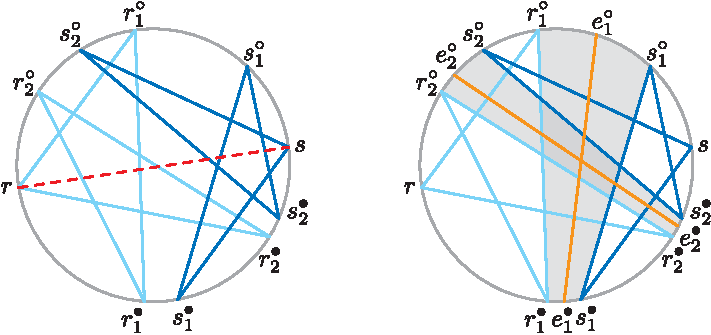
\includegraphics[scale=.8]{combisector}}
	\caption{The common bisector~$(r,s)$ of two $2$-stars~$R$ and~$S$ (left) and a $2$-crossing crossing~$(r,s)$. Picture adapted from~\cite[Fig.~4]{PilaudSantos-multitriangulations}.}
	\label{fig:combisector}
\end{figure}

\begin{lemma}[{\cite[Lems.~3.6 \& 3.7]{PilaudSantos-multitriangulations}}]
\label{lem:crossingCommonBisector}
Consider two $k$-stars~$R$ and~$S$ and a $k$-crossing~$E$ whose union is $(k+1)$-crossing free, with the notations described above and illustrated in \cref{fig:combisector}. Then, for any~$i \in [k]$,
\[
r \cl r^\bullet_i \cle e^\bullet_i \cle s^\bullet_i \cl s \cl s^\circ_i \cle e^\circ_i  \cle r^\circ_i \cl r.
\]
In other words, the diagonals $r_i$ of~$R$ and~$s_i$ of~$S$ are parallel and the diagonal~$e_i$ must be in between $r_i$ and~$s_i$.
\end{lemma}

%%%

\subsubsection{Flipping a $k$-relevant diagonal}

The observations of the previous section enables us to prove the following statement.
It is illustrated on \cref{fig:flip}.


\begin{figure}
	\capstart
	\centerline{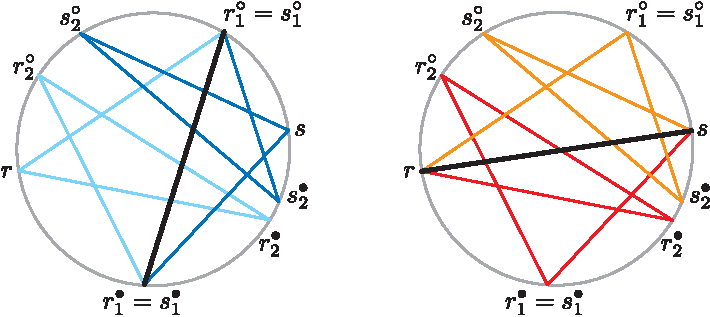
\includegraphics[scale=.8]{flip}}
	\caption{Flipping a diagonal common to two $k$-stars into their common bisector. Picture adapted from~\cite[Fig.~5]{PilaudSantos-multitriangulations}.}
	\label{fig:flip}
\end{figure}


\begin{lemma}[{\cite[Lem.~3.8]{PilaudSantos-multitriangulations}}]
\label{lem:flip}
Let~$R$ and~$S$ be two $k$-stars of a $(k+1)$-crossing-free collection~$F$ of diagonals.
Label the vertices of~$R$ by~$r \cl r^\bullet_1 \cl \dots \cl r^\bullet_k \cl r^\circ_1 \cl \dots \cl r^\circ_k$ and the vertices of~$S$ by~$s \cl s^\circ_1 \cl \dots \cl s^\circ_k \cl s^\bullet_1 \cl s^\bullet_k$ such that~$f = (r,s)$ is the common bisector of~$R$ and~$S$.
If~$R$ and~$S$ share a common diagonal~$e$, then
\begin{enumerate}[(i)]
\item there exists~$i \in [k]$ such that~$e = r_i = s_i$,
\item $F \symdif \{e,f\}$ is $(k+1)$-crossing-free (where~$\symdif$ denotes the symmetric difference),
\item in $F \symdif \{e,f\}$, the vertices~$r, r^\circ_1, r^\bullet_1, \dots, r^\circ_i = s^\circ_i, s^\bullet_{i+1}, s^\circ_{i+1}, \dots, s$ form a $k$-star~$X$ while the vertices~$s, s^\bullet_1, s^\circ_1, \dots, s^\bullet_i = r^\bullet_i, r^\circ_{i+1}, r^\bullet_{i+1}, \dots, r$ form a $k$-star~$Y$,
\item $X$ and~$Y$ share a common diagonal~$f$ and have common bisector~$e$.
\end{enumerate}
\end{lemma}

\begin{proof}
Again, the proof of~\cite[Lem.~3.8]{PilaudSantos-multitriangulations} applies to the infinite case.
The main argument is that any $k$-crossing of~$E$ that prevents~$e$ being in~$E$ contains the diagonal~$f$ by~\cref{lem:crossingCommonBisector}, so that~$e$ can be safely added to~$E \ssm \{f\}$.
\end{proof}

We are finally ready to prove \cref{thm:structureInfinite}\,(3).

\begin{corollary}
For any \ef \ktg~$T$ of a tidy polygon~$P$ and any $k$-relevant diagonal~$e$ of~$T$, there exists a unique diagonal~$f$ not in~$T$ such that~$T \symdif \{e,f\}$ is another $k$-triangulation. The diagonal~$f$ only depend on the two $k$-stars of~$T$ containing~$e$.
\end{corollary}

\begin{proof}
By \cref{coro:diagonalInStars}, the diagonal~$e$ is contained in two $k$-stars~$R$ and~$S$ of~$T$.
By \cref{thm:uniqueCommonBisector}, the $k$-stars~$R$ and~$S$ have a unique common bisector~$f$.
By \cref{lem:flip}, the collection of diagonals~$T \symdif \{e,f\}$ is $(k+1)$-crossing-free.
Finally, $T \symdif \{e,f\}$ must be maximal: otherwise, it is contained in a $k$-triangulation~$T'$ and~$T' \symdif \{e,f\}$ is $(k+1)$-crossing-free and properly contains~$T$.
\end{proof}

%%%

\subsubsection{Flattening a boundary $k$-star, inflating a boundary $k$-crossing}

~

\begin{figure}[h]
  \centering
  \begin{subfigure}[b]{.48\textwidth}
	\centering
	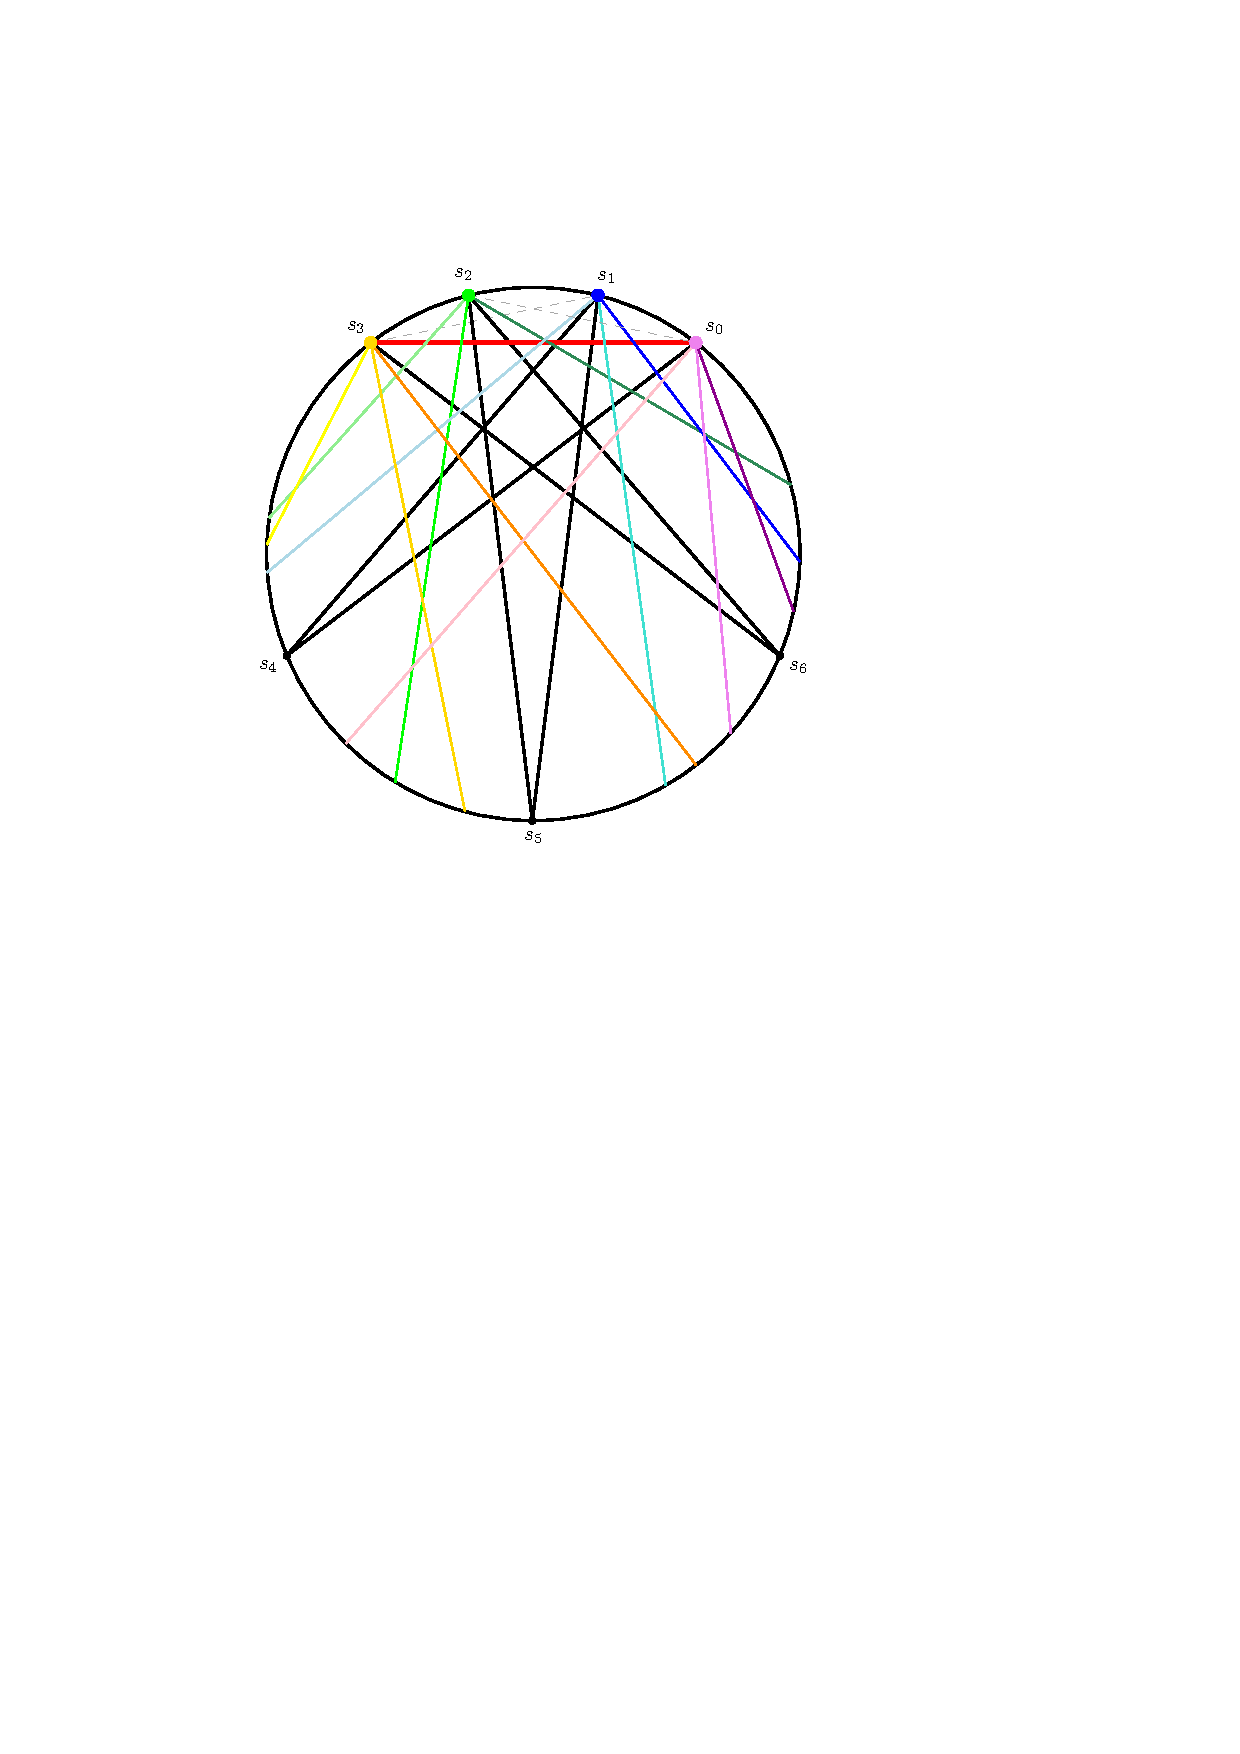
\includegraphics[width=\textwidth,page=1]{exFlattening}
  \end{subfigure}
  \begin{subfigure}[b]{.48\textwidth}
    \centering
    \includegraphics[width=\textwidth,page=2]{exFlattening}
  \end{subfigure}
  \caption{Illustrations of the flattening of a boundary $k$-star, with $k=3$.}
  \label{fig:exProofStar}
\end{figure}

%%%%%%%%%%%%%%%%%%%%%%%%%%%%%%%%%%%%%%

\newpage
\section{Multitriangulations of a general surface}
\label{sec:multitriangulationsSurfaces}

The objective of this section is to provide a consistent definition of multitriangulations of surfaces and to discuss some of their properties.
The naive definition (no $(k+1)$-subset of pairwise crossing arcs on the surface) yields poorly behaved objects, so we have to use the universal cover of the surface.
 
%%%%%%%%%%%%

\subsection{Surfaces and their universal covers}

We start with the equivalents of vertices and diagonals on a surface.

\begin{definition}
Consider a connected surface~$\surface$ with boundary and a set~$V$ of marked points on the boundary.
An \defn{arc} of~$\surface$ is a curve on~$\surface$ connecting two points of~$V$ and whose interior is disjoint from the boundary of~$\surface$.
We consider arcs up to homotopy relative to their endpoints in~$\surface$ and we disallow arcs homotopic to a boundary segment of~$\surface$.
\end{definition}

%\begin{remark}
%We could also consider the case of a surface with no marked points on some boundaries. Be careful that the definition of $k$-relevant, $k$-boundary and $k$-irrelevant diagonals are not clear anymore in that case.
%\end{remark}

In this section, we will use the representation of surfaces as quotients of the hyperbolic plane by Fuchsian groups.
As we only use the combinatorial aspects of this description, we take the liberty to remain quite informal on this representation.
Any surface~$\surface$ can be constructed from a polygon~$P$ by glueing some of its edges (the unglued edges of the polygon form the boundary of the surface~$\surface$).
When the surface has genus~$g > 1$ and no boundary, there is a subgroup~$\Gamma$ of isometries of the hyperbolic disk~$\disk$ so that this polygon~$P$ is the fundamental domain of~$\Gamma$, the surface~$\surface$ is isomorphic to the quotient~$\disk/\Gamma$, and the disk~$\disk$ is the universal cover of the surface~$\surface$.
When the surface has boundaries, we use a similar representation.
We embed $P$ in the hyperbolic disk~$\disk$ and we consider the subgroup~$\Gamma$ of isometries of the hyperbolic disk~$\disk$ generated by the identifications of the edges of~$P$ dictated by the surface~$\surface$.
The universal cover of the surface~$\surface$ is then the part~$\bar\surface$ of the hyperbolic disk~$\disk$ tiled by all images of~$P$ by~$\Gamma$.
We denote by~$\pi: \bar\surface \to \surface$ the projection from the universal cover~$\bar\surface$ down to the surface~$\surface$.
This representation is illustrated for instance in \cref{fig:torusGroup}.

\begin{figure}
	\capstart
	\centerline{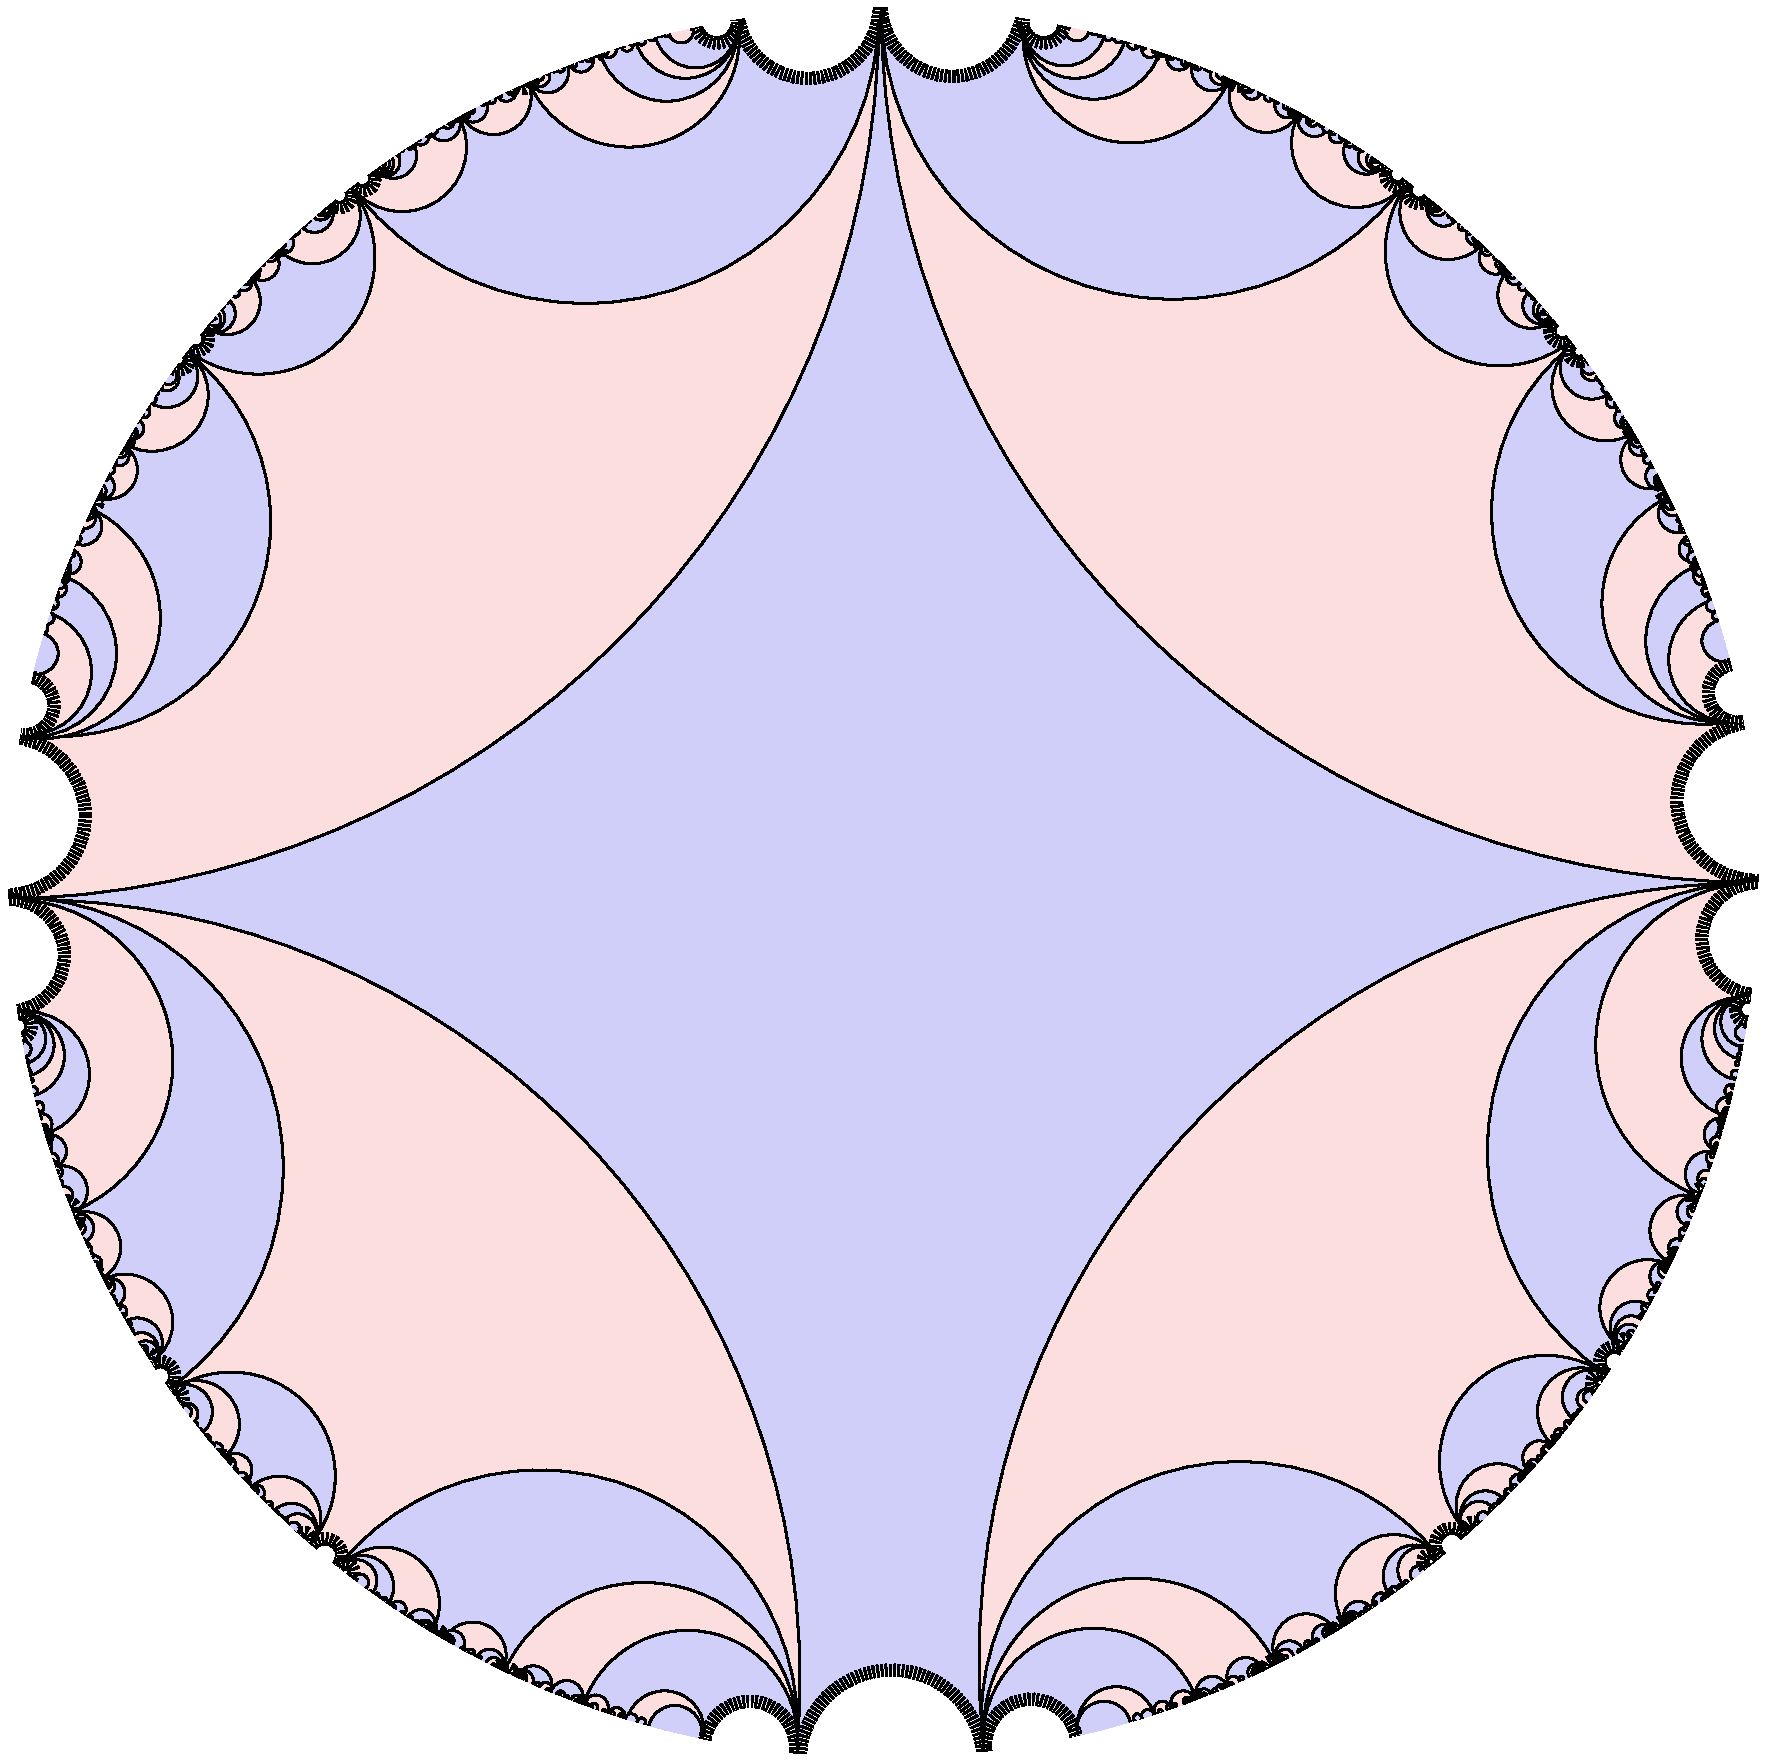
\includegraphics[scale=.42]{torus/torusGroup}}
	\caption{The torus with one hole, represented as the quotient of its universal cover by a Fuchsian group.}
	\label{fig:torusGroup}
\end{figure}

%%%%%%%%%%%%

\subsection{$k$-crossings, $k$-stars and $k$-triangulations on surfaces}

We now define $k$-crossings, $k$-stars and $k$-triangulations on a surface~$\surface$ by projection down to~$\surface$ of the same objects in the universal cover~$\bar\surface$.

\begin{definition}
\label{def:crossingsStarsTriangulationsSurfaces}
Let~$\surface$ be a surface, let~$\Gamma$ the corresponding subgroup of isometries of the hyperbolic disk~$\disk$, let~$\bar\surface$ be its universal cover, and let~$\pi : \bar\surface \to \surface$ be the canonical projection.
\begin{enumerate}[(i)]
\item A \defn{$k$-crossing} on~$\surface$ is the projection~$\pi(\bar a_1), \dots, \pi(\bar a_k)$ of a $k$-crossing~$\bar a_1, \dots, \bar a_1$ of~$\bar\surface$.
\item A \defn{$k$-star} on~$\surface$ is the projection~$\pi(\bar S)$ of a $k$-star~$\bar S$ of~$\bar\surface$.
\item A \defn{$k$-triangulation} of~$\surface$ is the projection~$\pi(\bar T)$ of a $\Gamma$-periodic $k$-triangulation~$\bar T$ of~$\bar\surface$.
\end{enumerate}
\end{definition}

\begin{remark}
Be careful: a $k$-crossing on~$\surface$ is NOT a collection of pairwise crossing arcs of~$\surface$. Namely, there are collections of pairwise crossing arcs of~$\surface$ which do not admit pairwise crossing representatives in~$\bar\surface$. The simplest examples are self-crossing arcs, whose representation may not be self-crossing. 
%Further examples are given in \cref{fig:notkcrossing}.
%\vincent{Todo.}
\end{remark}

\begin{remark}
By definition, a $k$-triangulation of a surface~$\surface$ is a maximal collection of arcs of~$\surface$ with no $(k+1)$-crossing (in the sense of \cref{def:crossingsStarsTriangulationsSurfaces}\,(ii)).
We conjecture that this characterizes $k$-triangulations of~$\surface$.
Indeed, note that the fiber of such a maximal $(k+1)$-crossing free collection~$T$ of arcs of~$\surface$ is always by definition a $(k+1)$-crossing free collection~$\bar T$ of diagonals of~$\bar\surface$, but it is not clear to us that it is always maximal in~$\bar\surface$.
\end{remark}

\begin{lemma}
\label{lem:surfaceToPolygon}
If~$T$ is a $k$-triangulation of~$\surface$, then its covering $k$-triangulation~$\bar T$ of~$\bar\surface$ is an \ef $k$-triangulation of a tidy polygon.
\end{lemma}

\begin{proof}
For any diagonal~$\bar a$ in~$\bar T$, the sequence~$\bar a_1, \dots, \bar a_p$ of arcs crossed by~$\bar a$ projects down to the sequence~$\pi(\bar a_1), \dots, \pi(\bar a_p)$ crossed by~$\pi(\bar a)$. Thus, $\bar a$ crosses only finitely many arcs and~$\bar T$ is \ef.
The polygon is tidy since each marked point in~$\bar\surface$ has for predecessor (resp.~successor) the previous (resp.~next) point along the boundary of~$\surface$. 
\end{proof}

\begin{figure}[b]
	\capstart
	\centerline{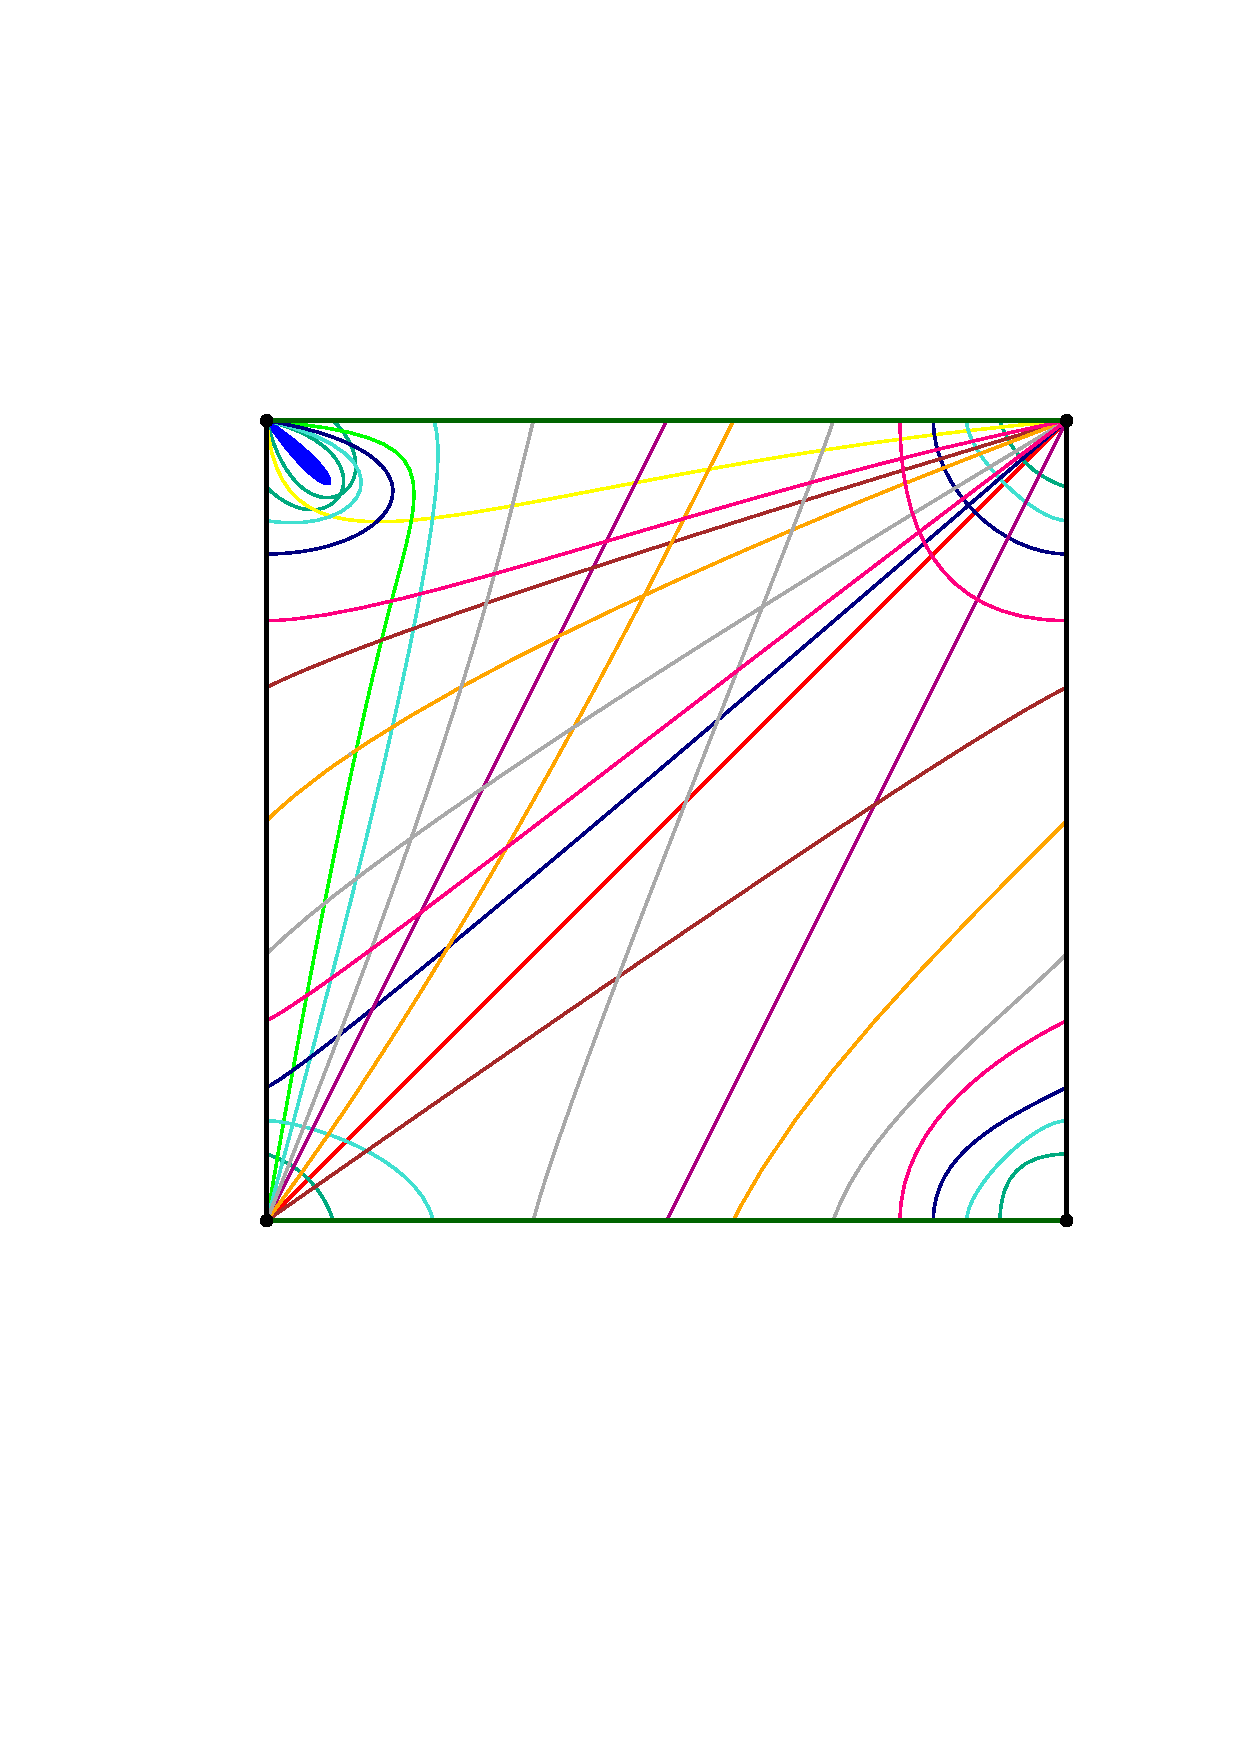
\includegraphics[scale=.42]{exTorusSquare}}
	\caption{A $2$-triangulation of a torus with a hole (in blue), whose universal cover is represented in \cref{fig:torusEdges}.}
	\label{fig:torus}
\end{figure}

%For an arc~$a$ on the surface~$\surface$, we denote by~$\bar a \eqdef \pi^{-1}(a)$ its fiber under the projection~$\pi$.
%We call \defn{representative} of the arc~$a$ in the universal cover~$\bar\surface$ any arc~$\tilde a$ in~$\bar\surface$ such that~$\pi(\tilde a) = a$.
%For a collection~$T$ of arcs, we also denote by~$\bar T \eqdef \pi^{-1}(T) = \bigcup_{a \in T} \bar a$.
%
%\begin{definition}
%A \defn{$k$-crossing} on~$\surface$ is a collection~$a_1, \dots, a_k$ (possibly with repetition) of $k$ arcs of~$\surface$ which admit pairwise crossing representatives~$\tilde a_1, \dots, \tilde a_k$ in the universal cover~$\bar\surface$.
%A \defn{$k$-triangulation} of~$\surface$ is an inclusion maximal set of arcs of~$\surface$ with no $(k+1)$-crossing.
%\end{definition}
%
%\begin{example}
%
%\end{example}
%
%Our main tool to study $k$-triangulations of a surface~$\surface$ is to study their universal cover.
%
%\begin{proposition}
%\label{prop:surfaceToPolygon}
%Let~$T$ be a $k$-triangulation of a surface~$\surface$ and let~$\bar T$ denote the corresponding set of arcs in the universal cover~$\bar\surface$.
%Then~$\bar T$ is an \ef $k$-triangulation of a tidy polygon.
%\end{proposition}
%
%\begin{proof}
%
%\end{proof}


%%%%%%%%%%%%

\newpage
\subsection{Structural properties}

We now explore structural properties of $k$-triangulations of a surface.
Our approach is again through $k$-stars.

%\begin{definition}
%A \defn{$k$-star} on a surface~$\surface$ is the projection on~$\surface$ of a $k$-star of the universal cover~$\bar\surface$.
%\end{definition}

%There are other equivalent ways to define $k$-stars on the surface.
%\vincent{Which ones?}
%For instance, one can define an angle of a collection~$T$ of arcs on~$\surface$ as a pair of consecutive arcs around a common vertex.
%A $k$-star of~$\surface$ can then be defined as a cyclic collection of $2k+1$ arcs~$a_0, \dots, a_{2k+1}$ arcs of~$\surface$ such that any two consecutive ones~$a_i$ and~$a_{i+1}$ (including~$a_{2k+1}$ and~$a_0$) form an angle of~$\surface$.

\begin{theorem}
\label{thm:arcInStar}
For any $k$-triangulation~$T$ of a surface~$\surface$, each $k$-relevant (resp.~$k$-boundary, resp.~$k$-irrelevant) arc of~$T$ is contained in precisely two (resp.~one, resp.~no) $k$-stars of~$T$.
\end{theorem}

\begin{proof}
Let~$\bar T$ be collection of arcs of~$\bar\surface$ which projects to the $k$-triangulation~$T$ of~$\surface$.
Since~$\bar T$ is an \ef $k$-triangulation of a tidy polygon by \cref{lem:surfaceToPolygon}, we can apply \cref{thm:structureInfinite} and obtain that each $k$-relevant (resp.~$k$-boundary, resp.~$k$-irrelevant) arc of~$\bar T$ is contained in precisely two (resp.~one, resp.~no) $k$-stars of~$\bar T$.
The statement thus follows by projection of~$\bar T$ to~$T$.
\end{proof}

\begin{figure}[h]
	\capstart
	\centerline{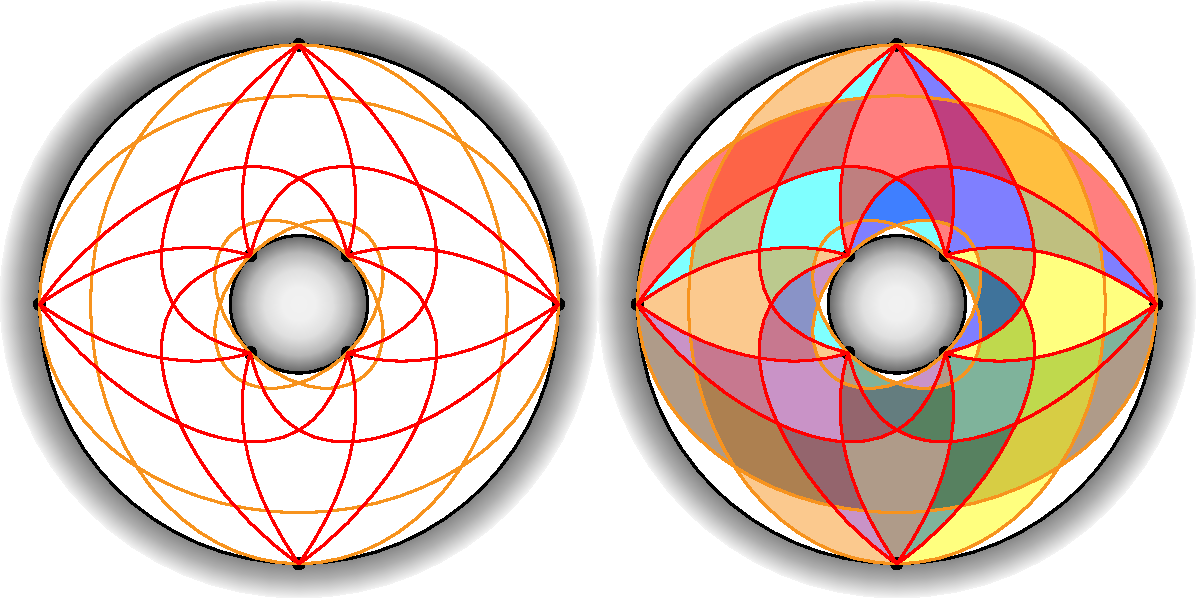
\includegraphics[scale=.5]{2triangCylinderStars}}
	\caption{A $2$-triangulation of a cylinder, where $2$-relevant arcs are red while $2$-boundary arcs are orange (left) and its decomposition into $2$-stars (right).}
	\label{fig:starsSurface}
\end{figure}

Using \cref{thm:arcInStar}, we obtain the number of $k$-stars and $k$-relevant arcs in a $k$-triangulation.
We start with the case of surfaces with at least one marked point on each connected component, for which we argue by a cutting argument.

\begin{theorem}
\label{thm:countingStarsArcsSurface}
Consider a surface~$\surface$ of genus~$g$ with~$b$ boundaries and~$n$ marked points, such that there is at least one marked point on each boundary.
Then any \ktg of~$\surface$  has precisely $n + 2k(2g + b - 2)$ $k$-stars and $kn + k(2k + 1)(2g + b - 2)$ $k$-relevant arcs.
\end{theorem}

\begin{proof}
%There are various possible proofs of this statement, none of them is really clean at the moment.
%
%The first (original) proof is based on cutting along arcs.
We sketch a proof based on cutting along arcs.
Start from a $k$-triangulation~$T$ of a surface~$\surface$ with at least~$2k+1$ marked points, genus~$g$ and $b$ boundaries.
If~$T$ has no $k$-relevant arc, then~$T$ is the complete graph on $2k+1$ vertices, has a single $k$-star, and $\surface$ is a disk.
Otherwise, pick an arbitrary $k$-relevant arc~$a$ of~$T$.
Cut along~$a$, create $k-1$ new marked points on each side of~$a$, and rearrange the branches of the $k$-stars that cross~$a$ to these new marked points (there is a unique way to do this rearrangement).
This operation, illustrated in \cref{fig:cutSurface}, is easier to see on the disk, and can then be extended to surfaces using the universal cover.
%
\begin{figure}[t]
	\capstart
	\centerline{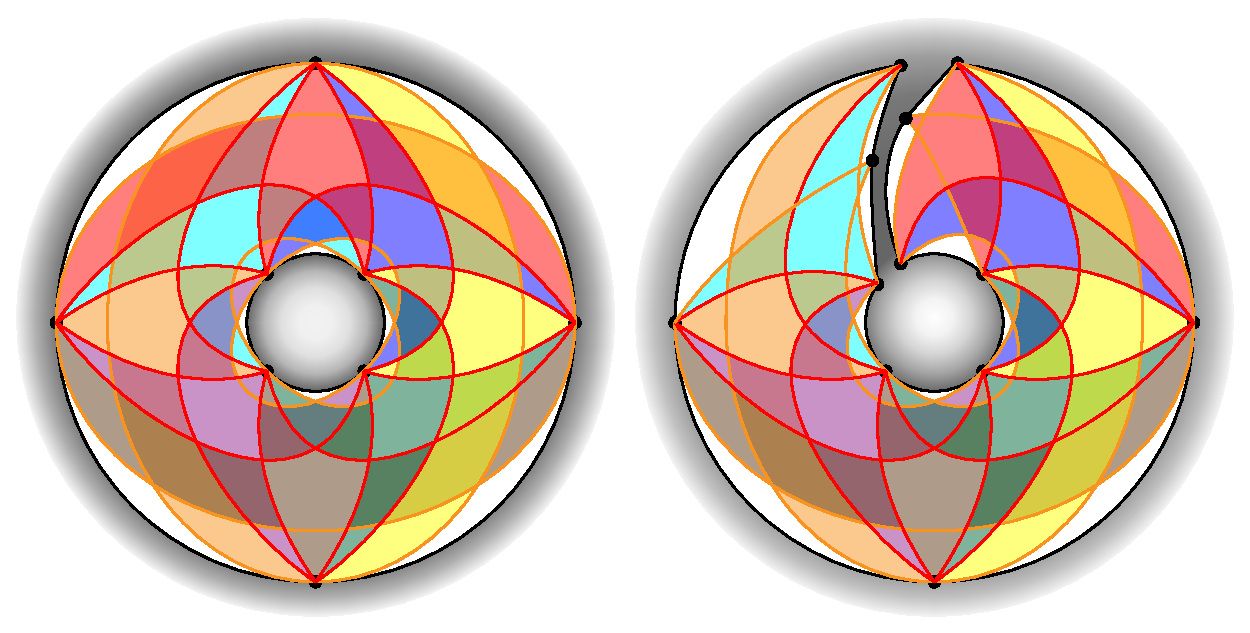
\includegraphics[scale=.5]{2triangCylinderCut}}
	\caption{Cutting a $2$-triangulation of a cylinder along a $2$-relevant arc.}
	\label{fig:cutSurface}
\end{figure}
%
We obtain a new $k$-triangulation~$T'$ on a new surface~$\surface'$ (not necessarily connected).
Note that
\begin{enumerate}
\item the $k$-triangulations~$T$ and~$T'$ have the same number of $k$-stars,
\item the surface~$\surface'$ has $n' = n+2k$ marked points (as we have duplicated the endpoints of~$a$ and we have created $2k-2$ new marked points),
\item the genus~$g'$ and number of boundaries~$b'$ of the surface~$\surface'$ depend on the choice of~$a$:
	\begin{itemize}
	\item if the endpoints of~$a$ belong to the same connected component of~$\surface$, then we cut a handle and thus~$g' = g-1$ and $b' = b+1$,
	\item if the endpoints of~$a$ belong to distinct connected components of~$\surface$, then we cut a border and thus~$g' = g$ and~$b' = b-1$.
	\end{itemize}
	But in both cases, $2g'+b' = 2g+b-1$.
\end{enumerate}
We conclude that $T'$ has indeed $n + 2k(2g + b -2) = n' + 2k(2g' + b - 2)$ $k$-stars.

%\medskip
%I am working on another proof, but I can't yet make it work correctly.
\medskip
Once we know the number of $k$-stars, the number of $k$-relevant arcs immediately follows by double counting.
Indeed, since
\begin{itemize}
\item each $k$-relevant arc belongs to two $k$-stars while each $k$-boundary arc belongs to one $k$-star,
\item each $k$-star contains $2k+1$ arcs which are all either $k$-relevant of $k$-boundary,
\item there are precisely $n$ $k$-boundary arcs,
\end{itemize}
we obtain that the number $s$ of $k$-stars and the number $r$ of $k$-relevant arcs in a $k$-triangulation are related by
\(
2r + n = (2k+1) s
\)
from which we derive that
\[
r = \big( (2k+1)s-n \big)/2 = kn + k(2k + 1)(2g + b - 2).
\qedhere
\]
\end{proof}

We can now obtain the number of $k$-stars and $k$-relevant arcs for arbitrary surfaces.

\begin{corollary}
\label{coro:countingStarsArcsSurface}
Consider a surface~$\surface$ of genus~$g$ with~$b$ boundaries and~$n$ marked points, such that $b^\circ$ boundaries have no marked points.
Then any \ktg of~$\surface$  has $n + 2k(2g + b - 2) - b^\circ$ $k$-stars and $kn + k(2k + 1)(2g + b - 2) - kb^\circ$ $k$-relevant arcs.
\end{corollary}

\begin{proof}
Let~$T$ be a $k$-triangulation of~$\surface$, and denote by $s$ its number of $k$-stars and by $r$ its number of $k$-relevant arcs.
We can add to~$T$ a marked point, a $k$-star and $k$ $k$-relevant arcs to enclose each boundary of~$\surface$ with no marked point.
The resulting surface~$\tilde\surface$ has genus~$\tilde g \eqdef g$, $\tilde b \eqdef b$ boundaries and $\tilde n \eqdef n+b^\circ$ marked points and there is at least one marked point on each boundary.
The resulting $k$-triangulation~$\tilde T$ has~$\tilde s \eqdef s+b^\circ$ $k$-stars and~$\tilde r \eqdef r+kb^\circ$ $k$-relevant arcs.
%By \cref{thm:countingStarsArcsSurface}, we obtain that~$\tilde s = \tilde n + 2k(2 \tilde g + \tilde b - 2)$ and $\tilde  r = k \tilde n + k(2k + 1)(2 \tilde g + \tilde b - 2)$.
We conclude by \cref{thm:countingStarsArcsSurface}.
\end{proof}

\begin{figure}[b]
	\capstart
	\centerline{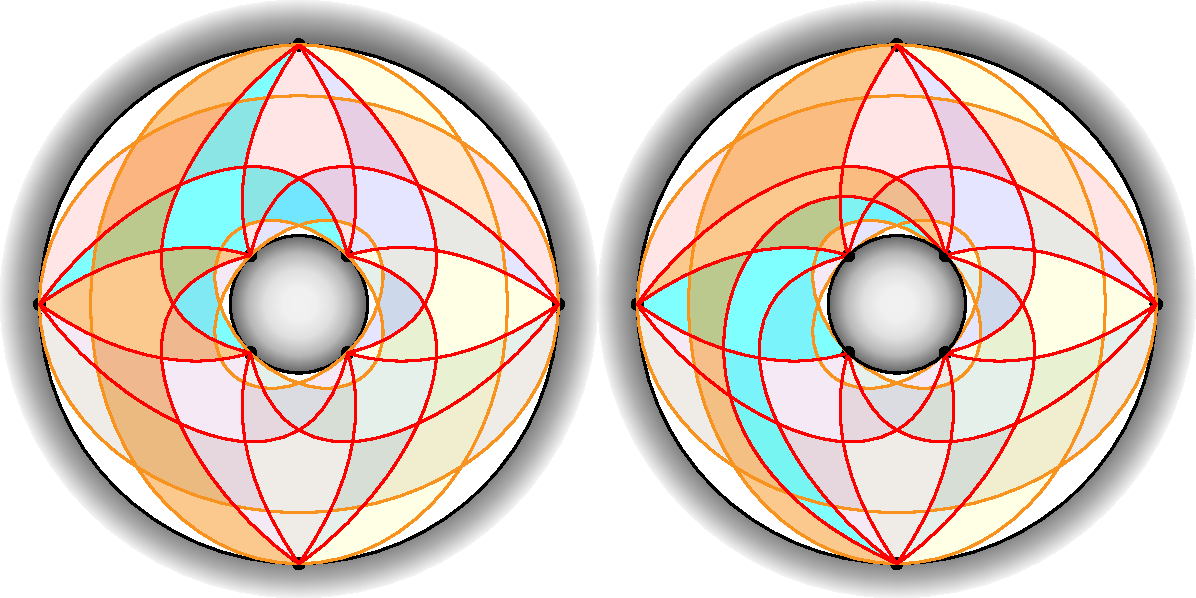
\includegraphics[scale=.5]{2triangCylinderFlip}}
	\caption{A flip of a $2$-relevant arc in a $2$-triangulation of a cylinder.}
	\label{fig:flipSurface}
\end{figure}

%\begin{remark}
%\begin{itemize}
%\item \cite[Lem.~7.10]{PilaudSantos-multitriangulations}: Any $k$-triangulation of the $n$-gon contains at most $k(n-2p-1)$ $p$-relevant diagonals. Extension for surfaces.
%\item flip graph connected? Increasing flip graph? Is it a lattice? (use bracket vectors)
%\item duality? Line space of the surface?
%\item punctures?
%\end{itemize}
%\end{remark}

Our last structural property concerns flips in $k$-triangulations of surfaces.
The remaining of this note discusses the following conjecture.

\begin{conjecture}
\label{conj:generalFlip}
Any $k$-relevant arc of a $k$-triangulation on a surface can be flipped.
\end{conjecture}

%Consider a $k$-triangulation~$T$ of a surface~$\surface$.
%Let~$\bar T$ be the corresponding infinite $k$-triangulation of the universal cover~$\bar \surface$.
%We want to show that any $k$-relevant arc~$a$ of~$T$ is flippable.
To flip a $k$-relevant arc~$a$ of the $k$-triangulation~$T$ of a surface~$\surface$, the natural idea is to flip sequentially all copies~$\bar a$ of the arc~$a$ in the $k$-triangulation~$\bar T$ of the universal cover~$\bar\surface$.
However, this only works if, at any point of this procedure, the flip of any copy~$\bar a$ in~$\bar T$ does not modify the flip of the other copies of~$a$ in~$\bar T$.
We say that the flip of~$a$ in~$T$ is \defn{sequential} when this procedure works, and \defn{non-sequential} otherwise.

\begin{example}
For instance, all flips in the $2$-triangulation of \cref{fig:torusEdges} are sequential.
We will see examples of non-sequencial flips in \cref{sec:halfCylinder}.
\end{example}

Our approach to \cref{conj:generalFlip} would be to show that non-sequential flips in $k$-triangulations of any surface~$\surface$ just boil down to non-sequential flips of $k$-triangulations of a half-cylinder~$\cylinder$.
For this, consider an arc~$a$ of a $k$-triangulation~$T$ of~$\surface$, and let~$S,S'$ be the two $k$-stars of~$T$ containing~$a$.
We distinguish two cases:
\begin{itemize}
\item If~$S$ and~$S'$ are distinct $k$-stars of~$T$, then $a$ appears only once in~$S$ and in~$S'$. Consider a copy~$\bar a$ of~$a$ in~$\bar T$ and the copy~$\bar S$ (resp.~$\bar S'$) of~$S$ (resp.~$S'$) in~$\bar T$ containing~$\bar a$. Remember from \cref{sec:infiniteMultitriangulations} that the flip of~$\bar a$ in~$\bar T$ only depends on and only modifies the two $k$-stars~$\bar S$ and~$\bar S'$. Since~$\bar a$ is not contained in any other copy of~$S$ and~$S'$ in~$\bar T$, the flip of~$\bar a$ in~$\bar T$ does not modify the flip of the other copies of~$a$ in~$\bar T$. Therefore the flip is sequential.
\item Assume now that~$S = S'$ so that~$a$ appears twice in~$S$. Let~$\bar a$ and~$\bar a'$ be two copies of~$a$ in a copy~$\bar S$ of~$S$ in~$\bar T$. Let~$\gamma \in \Gamma$ be the isomorphism of~$\bar\surface$ such that~$\gamma(\bar a) = \bar a'$. We consider the collection~$\bar U$ of arcs of the $k$-stars~$\gamma^i(\bar S)$ for~$i \in \Z$. Perform all identifications of two consecutive vertices of~$\bar U$ that do not uncross any pairs of arcs of~$\bar U$. These identifications can be performed in any order. The result~$\bar V$ is a $k$-triangulation of an infinite polygon whose isomorphism group is generated by~$\gamma$. Therefore, $\bar V$ is a covering of a $k$-triangulation~$V$ of a cylinder~$\cylinder$.
\end{itemize}

\begin{conjecture}
\label{conj:decompCylinder}
The procedure described above leads to a $k$-triangulation~$\tilde T$ of a half-cylinder.
Moreover, one can totally understand the flips in the $k$-triangulation~$T$ of the surface~$\surface$ from the flips in the $k$-triangulation~$\tilde T$ of the half-cylinder.
\end{conjecture}

Although this approach is not yet settled, we believe that our presentation motivates to study in details the $k$-triangulations of the half-cylinder, which is the purpose of the remaining of the paper.

%%%%%%%%%%%%%%%%%%%%%%%%%%%%%%%%%%%%%%

\section{Multitriangulations of the half-cylinder}
\label{sec:halfCylinder}

This section is devoted to multitriangulations of half-cylinders, defined as follows.

\begin{definition}
A \defn{half-cylinder} is a cylinder with some marked points on the lower boundary, but no point on the upper boundary.
\end{definition}

As mentioned, the study of multitriangulations of half-cylinders has two relevant purposes:
\begin{itemize}
\item they provides examples of non-sequencial flips,
\item assuming \cref{conj:decompCylinder}, it provides the prototype to understand all non-sequencial flips of $k$-triangulations of surfaces.
\end{itemize}

%\begin{figure}
%\label{fig:saturatedHC2}
%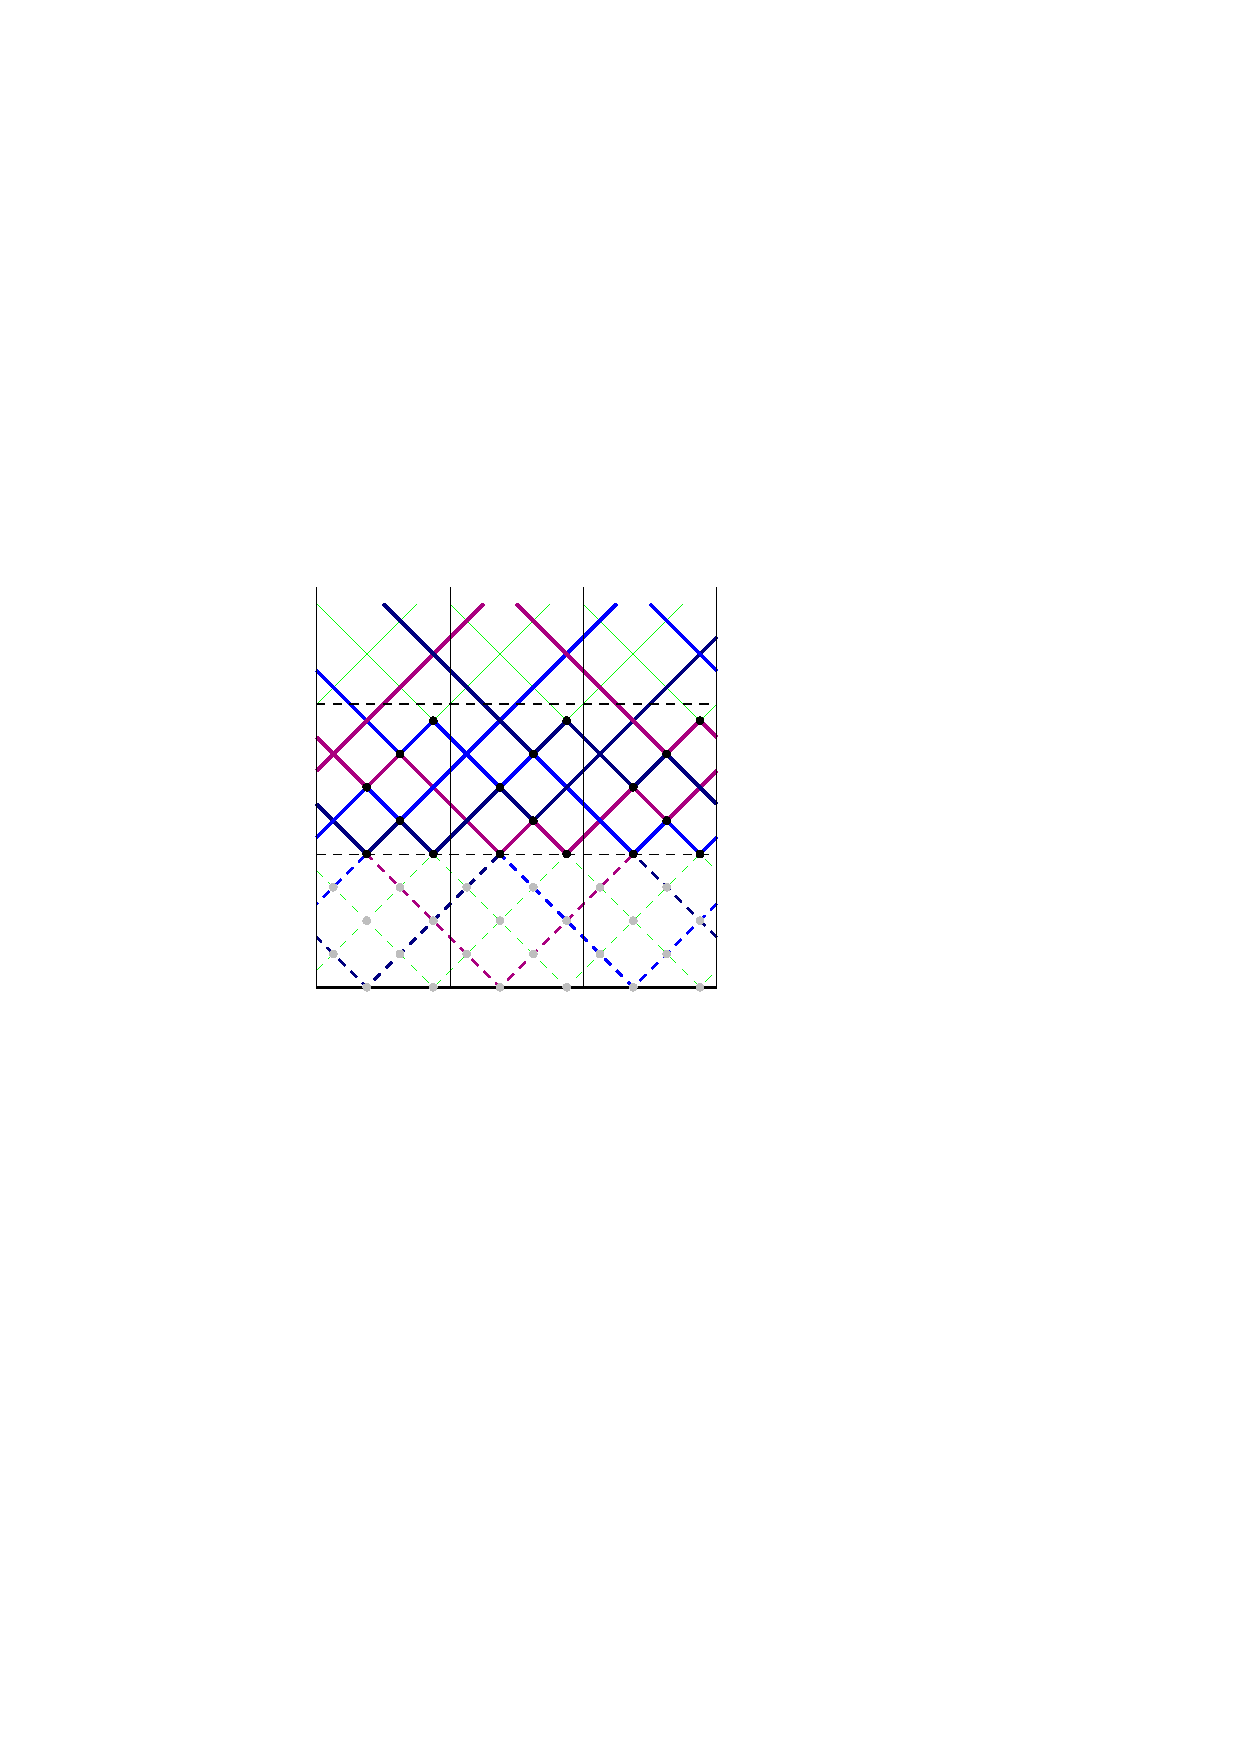
\includegraphics[scale=1]{saturatedHC}
%\caption{representation...}
%\end{figure}

%%%%%%%%%%%%

\subsection{Half-cylinder with $2$ marked points}

We start with the case of multitriangulations of the half-cylinder with only two points on the lower boundary.
This case already provides relevant examples of non-sequencial flips that will enable us to settle some conventions of representations (see \cref{fig:nonsequential,fig:nonsequentialVHrep}).

Consider the half-cylinder~$\cylinder$ with two points~$\{u,v\}$ on one boundary and none on the other.
Its universal cover~$\bar\cylinder$ is an infinite band, with points~$u_j$ and~$v_j$ for~$j \in \Z$ alternating on one boundary (so that~$u_j+1 = v_j = u_{j+1}-1$).
See \cref{fig:nonsequential}.

For~$k \ge 1$ and a word~$w \eqdef w^1 \dots w^k  \in \{u,v\}^k$, consider a set~$\bar T_w$ of diagonals of~$\bar\cylinder$ formed by
\begin{itemize}
\item the diagonals~$\bar a_w^i \eqdef (w^i_j, w^i_j+k+i)$ for all~$i \in [k]$ and~$j \in \Z$,
\item all $k$-boundary and $k$-irrelevant diagonals~$(\epsilon_j, \epsilon_j+i)$ for~$i \in [k]$, $\epsilon \in \{u,v\}$ and~$j \in \Z$.
\end{itemize}
For instance, we have represented the sets~$\bar T_{uvu}$ and~$\bar T_{uuu}$ in \cref{fig:nonsequential}.

\begin{figure}
	\capstart
	\includegraphics[page=2, scale=.5, clip, trim=15cm 0cm 17cm 0cm]{FNSk3p2} \\[.5cm]
	\includegraphics[page=3, scale=.5, clip, trim=15cm 0cm 17cm 0cm]{FNSk3p2}
	\caption{Two $3$-triangulations~$\bar T_{uvu}$ (top) and~$\bar T_{uuu}$ (bottom) of a half-cylinder related by a non-sequential flip. The diagonal~$u_i v_{i+2}$ is flipped to the diagonal~$v_i u_{i+3}$. These diagonals belong to two consecutive copies of the same $3$-star.}
	\label{fig:nonsequential}
\end{figure}

\begin{lemma}
\label{lem:noTwoDiagonalsEachLevel}
The sets
\begin{itemize}
\item $\set{(\epsilon_j, \epsilon_j+k+i)}{\epsilon \in \{u,v\} \text{ and } j \in \Z}$ for any~$i \in [k]$,
\item $\set{(\epsilon_j, \epsilon_j+k+i)}{j \in \Z}$ for any~$\epsilon \in \{u,v\}$ and~$i \ge k+1$,
\end{itemize}
all contain a $(k+1)$-crossing.
\end{lemma}

\begin{proposition}
For any~$k \ge 1$ and~$w  \in \{u,v\}^k$, the set~$\bar T_w$ is a $k$-triangulation of~$\bar\surface$.
\end{proposition}

\begin{proof}
The maximality is immediate from \cref{lem:noTwoDiagonalsEachLevel} or \cref{coro:countingStarsArcsSurface}.
To see that~$\bar T_w$ is $(k+1)$-crossing-free, we use the following strategy:
\begin{itemize}
\item the set of diagonals~$\set{(\epsilon_j, \epsilon_j+2k)}{j \in \Z}$ has no $(k+1)$-crossing for any~$\epsilon \in \{u,v\}$,
\item given any set~$D$ of pairwise crossing diagonals in~$\bar T_w$, we can construct a new set~$D'$ of pairwise crossing diagonals in~$\bar T_w$ by increasing the length of the smallest diagonal~$(u,v)$ of~$D$, provided this length is not~$2k$. Indeed, we just need to observe that the vertices~$u-1$ and~$v-1$ cannot be incident to diagonals of~$D$.
\qedhere
\end{itemize}
\end{proof}

\begin{corollary}
\label{coro:allkTriangCyclinder}
The set of $k$-triangulations of~$\bar\cylinder$ is~$\set{\bar T_w}{w \in \{u,v\}^k}$.
\end{corollary}

\begin{proof}
Any $(k+1)$-crossing free set of diagonals of~$\bar\cylinder$ is a subset of a certain~$\bar T_w$ by \cref{lem:noTwoDiagonalsEachLevel}.
\end{proof}

Consider now the projection~$\pi : \bar\cylinder \to \cylinder$. We denote by 
\begin{itemize}
\item $a_w^i$ the arc of~$\cylinder$ obtained by projection of any diagonal~$(w^i_j, w^i_j+k+1+i)$ of~$\bar\cylinder$ for~$j \in \Z$.
\item $T_w$ the $k$-triangulation of~$\cylinder$ obtained by projection of the $k$-triangulation~$\bar T_w$ of~$\bar\cylinder$.
\end{itemize}

\begin{proposition}
\label{prop:flip2halfCylinder}
%For any~$w \in \{u,v\}^k$ and~$i \in [k]$, the diagonal~$a_w^i$ of the $k$-triangulation~$T_w$ can be fli
For any~$w, w' \in \{u,v\}^k$ which only differ at position~$i \in [k]$, the $k$-triangulations~$T_w$ and~$T_w'$ are the only two $k$-triangulations~$\surface$ which contain~${T_w \ssm \{a_w^i\} = T_{w'} \ssm \{a_{w'}^i\}}$. In other words, any arc~$a_w^i$ in the $k$-triangulation~$T_w$ can be uniquely flipped.
\end{proposition}

\begin{proof}
By definition of~$T_w$ and~$T_{w'}$, we have~${T_w \ssm \{a_w^i\} = T_{w'} \ssm \{a_{w'}^i\}}$ so that the flip is possible.
It is unique by \cref{coro:allkTriangCyclinder}.
\end{proof}

\begin{remark}
The flip of $a_w^1$ is sequential (for the first flip, all points below $a_w^1$ are vertices of the $k$-star below~$a_w^1$ and we can determine which of these angles see each other; we have not worked out the other flips yet).
In contrast, the flip of~$a_w^i$ is not sequential for~$i \in \{2, \dots, k-1\}$ (since the common bisector is still of length~$k+1$).
\end{remark}

%%%%%%%%%%%%

\subsection{All half-cylinders}

We now consider an arbitrary half-cylinder~$\cylinder_n$ with $n$ points $(v_i)_{i \in \Z/n\Z}$ on the lower boundary and no point on the upper boundary. 
For a point~$v_i \in \cylinder_n$, we denote by~$(v_i^j)_{j \in \Z}$, its successive copies in the universal cover~$\overline{\cylinder_n}$ (which is an infinite band).
The objective of this section is to discuss the following conjectural extension of~\cref{prop:flip2halfCylinder}.

\begin{conjecture}
\label{conj:flipHalfCylinder}
Any arc of a $k$-triangulation of the half-cylinder~$\cylinder_n$ can be flipped.
\end{conjecture}

To approach this statement, we need to introduce a convenient representation of collections of arcs on the half-cylinder~$\cylinder_n$, illustrated in \cref{fig:nonsequentialVHrep}.

Let $A$ be a $(k+1)$-crossing-free set of $k$-irrelevant or $k$-boundary arcs of $\cylinder_n$ containing (at least) the $k$-boundary arcs of $\cylinder_n$, and $a$ be a $k$-relevant arc of $A$. We denote by $l_a$, $i_a$ and $j_a$ the length, and the indices of the left and right endpoints of $a$. Note that $l_a \ge k$ because $a$ is $k$-relevant, and $l_a \le kn$ because $A$ is $(k+1)$-crossing-free. Note also that $i_a+l_a-j_a=0$ (in $\Z/n\Z$) by definition.

\begin{figure}[b]
	\capstart
	\mbox{\includegraphics[page=6, scale=.5, clip, trim=21.2cm 0cm 24cm 6cm]{FNSk3p2} \quad \raisebox{1.7cm}{\includegraphics[page=4, scale=.5]{FNSk3p2}}} \\[.5cm]
	\mbox{\includegraphics[page=7, scale=.5, clip, trim=21.2cm 0cm 24cm 6cm]{FNSk3p2} \quad \raisebox{1.7cm}{\includegraphics[page=5, scale=.5]{FNSk3p2}}}
	\caption{The V (left) and H (right) representations of the $3$-triangulations of \cref{fig:nonsequential}.}
	\label{fig:nonsequentialVHrep}
\end{figure}

We represent $\cylinder_n$ by a cylindric grid $G$ of width $n$ and height $kn-n+1$, where each column, indexed by $\Z/n\Z$, represent a point, and each row, indexed by $[k,kn]$ represent an arc length.
We represent each arc $a$ of $A$ by a symbol $\bullet$ at position $(i_a,l_a)$ in $G$.
We associate a directed lattice to the grid $G$, made of an edge going from any point $(i,l)$ to the point $(i-1,l+1)$, and an edge from any point $(i,l+1)$ to the point $(i,l)$, for $l<kn$ and $i \in \Z/n\Z$, as well as an edge going from point $(i,kn)$ to point $(i,kn)$ for any $i \in \Z/n\Z$.
We naturally call these edges the \emph{upper outgoing}, \emph{upper ingoing}, \emph{lower outgoing}, \emph{lower ingoing} edges of a point. Note that points of the form $(i,k)$ have no lower edges.

A face of $A$ is made of a succession of \emph{top} arcs (that are above the face), and \emph{bottom} arcs (that are below the face). Around a face, their can be two consecutive bottom arcs, but no two consecutive top arcs. An angle between two bottom arcs is called \emph{upper angle}, an angle between a top and a bottom arcs is called \emph{lower angle}.
The \emph{counterclockwise tour} of a face $f$ of $A$ is computed by the following procedure. Start from any arc $a$ of $f$, and perform the following operation until you get back to this original arc~$a$.
\begin{enumerate}
\item If $a$ is a top arc, set $a$ to be longest arc starting from $v_{i_a}$ and having length less than $l_a$. Note that this is well defined because $A$ contains the $k$-boundary arcs, and a $k$-boundary arcs cannot be a top arc.
\item Else, if $a$ is a bottom arc, and $l_a$ is the maximum length of an edge ending on point~$v_{j_a}$, then set $a$ to be the longest arc starting on point~$v_{i_a}$.
\item Else, set $a$ to be the shorted arc ending on point $v_{j_a}$ and having length more than~$l_a$.
\end{enumerate}
If this procedure does not terminate, it means that the corresponding face is not finite, but rather infinite and periodic.

This procedure can easily be performed graphically in the grid representation, by following the edges of the lattice. Step $1$ corresponds to following lower outgoing edges until meeting a $\bullet$; step $3$ corresponds to following upper outgoing edges until meeting a $\bullet$; and step $2$ corresponds to following upper outgoing edges until reaching height $kn$, and then following lower outgoing edges until meeting a $\bullet$.
In the grid representation, this procedure necessarily ends with a cycle $C_f$.

We call \emph{drift} of the face~$f$ the integer $\delta_f$ equal the total length of top arcs of $C_f$ minus the total length of bottom arcs of $C_f$.
Then $f$ is finite if and only if $\delta_f=0$.

\begin{conjecture}
\label{conj:characterizationDots}
A collection $A$ of arcs of~$\cylinder_n$ is a $k$-triangulation if and only if it has $n-1$ faces, which all have drift $0$ and length $2k+1$.
\end{conjecture}

\begin{proof}[Tentative proof]
For the direct direction, assume that~$A$ is a $k$-triangulation of the half-cylinder~$\cylinder_n$.
By \cref{thm:structureInfinite,thm:arcInStar,coro:countingStarsArcsSurface}, it has $n-1$ $k$-stars, all of drift~$0$ and length $2k+1$.

Suppose now that $A$ has $n-1$ faces, all of drift $0$ and length $2k+1$. 
Counting the number of~$\bullet$, we obtain that $A$ is maximal by \cref{coro:countingStarsArcsSurface}.
The missing point is to prove that $A$ has no $(k+1)$-crossing.
\end{proof}

Let $T$ be a $k$-triangulation of $\cylinder_n$, let $S$ be a $k$-star of $T$, and let $a$ be an arc adjacent to $S$ on both sides.
Let $C_S$ be the cycle corresponding to $S$ in the grid representation.
Let $C_{S,d}^1$ be the subcycle of $C$ starting from the upper outgoing edge of $a$, and finishing at the lower ingoing edge of $a$.
Let $C_{S,d}^2$ be the subcycle of $C$ starting from the lower outgoing edge of $a$, and finishing at the upper ingoing edge of $a$.
The cycle $C$ is made of the succession of $C_{S,d}^1$ and $C_{S,d}^2$.

\begin{conjecture}
\label{conj:cycles}
The cycles $C_{S,d}^1$ and $C_{S,d}^2$ have exactly $2$ intersection points.
\end{conjecture}

\begin{proof}[Tentative proof]
The number of intersection points of two cycles on a cylinder is necessarily even. By definition, the $\bullet$ corresponding to $a$ is a point of intersection.
We thus just need to prove that there cannot be more than $2$ intersection points.
\end{proof}

\begin{proof}[Proof of \cref{conj:flipHalfCylinder} under \cref{conj:characterizationDots,conj:cycles}]
Let $T$ be a triangulation of $\cylinder_n$, and let $a$ be an arc of $T$.
If $a$ is adjacent to two different $k$-stars, then it can be flipped sequentially as discussed earlier.

If $a$ is adjacent twice to the same $k$-star, then denote by $a'$ the point of intersection between $C_{S,d}^1$ and $C_{S,d}^2$ which is not $a$.
Denote by $C_{S,d}^{1,1}$ and $C_{S,d}^{1,2}$ the subpaths of $C_{S,d}^1$ going from $a$ to $a'$, and from $a'$ to $a$.
Denote by $C_{S,d}^{2,1}$ and $C_{S,d}^{2,2}$ the subpaths of $C_{S,d}^2$ going from $a$ to $a'$, and from $a'$ to $a$.
The cycle $C$ is made of the cyclic concatenation of $C_{S,d}^{1,1}$, $C_{S,d}^{1,2}$, $C_{S,d}^{2,1}$, and $C_{S,d}^{2,2}$.

Now remove $a$ and add in $a'$. This creates a new face $S'$, corresponding in the grid representation to a cycle $C'$ made of the cyclic concatenation of $C_{S,d}^{1,1}$, $C_{S,d}^{2,2}$, $C_{S,d}^{2,1}$, and $C_{S,d}^{1,2}$.
Since $S'$ is made of the same paths as $S$, it as well has drift $0$ and length $2k+1$, so that what we obtain is a $k$-triangulation.
\end{proof}

%%%%%%%%%%%

\bibliographystyle{alpha}
\bibliography{multiTrig}

\end{document}
